% Options for packages loaded elsewhere
\PassOptionsToPackage{unicode}{hyperref}
\PassOptionsToPackage{hyphens}{url}
\documentclass[
]{book}
\usepackage{xcolor}
\usepackage{amsmath,amssymb}
\setcounter{secnumdepth}{5}
\usepackage{iftex}
\ifPDFTeX
  \usepackage[T1]{fontenc}
  \usepackage[utf8]{inputenc}
  \usepackage{textcomp} % provide euro and other symbols
\else % if luatex or xetex
  \usepackage{unicode-math} % this also loads fontspec
  \defaultfontfeatures{Scale=MatchLowercase}
  \defaultfontfeatures[\rmfamily]{Ligatures=TeX,Scale=1}
\fi
\usepackage{lmodern}
\ifPDFTeX\else
  % xetex/luatex font selection
\fi
% Use upquote if available, for straight quotes in verbatim environments
\IfFileExists{upquote.sty}{\usepackage{upquote}}{}
\IfFileExists{microtype.sty}{% use microtype if available
  \usepackage[]{microtype}
  \UseMicrotypeSet[protrusion]{basicmath} % disable protrusion for tt fonts
}{}
\makeatletter
\@ifundefined{KOMAClassName}{% if non-KOMA class
  \IfFileExists{parskip.sty}{%
    \usepackage{parskip}
  }{% else
    \setlength{\parindent}{0pt}
    \setlength{\parskip}{6pt plus 2pt minus 1pt}}
}{% if KOMA class
  \KOMAoptions{parskip=half}}
\makeatother
\usepackage{color}
\usepackage{fancyvrb}
\newcommand{\VerbBar}{|}
\newcommand{\VERB}{\Verb[commandchars=\\\{\}]}
\DefineVerbatimEnvironment{Highlighting}{Verbatim}{commandchars=\\\{\}}
% Add ',fontsize=\small' for more characters per line
\usepackage{framed}
\definecolor{shadecolor}{RGB}{248,248,248}
\newenvironment{Shaded}{\begin{snugshade}}{\end{snugshade}}
\newcommand{\AlertTok}[1]{\textcolor[rgb]{0.94,0.16,0.16}{#1}}
\newcommand{\AnnotationTok}[1]{\textcolor[rgb]{0.56,0.35,0.01}{\textbf{\textit{#1}}}}
\newcommand{\AttributeTok}[1]{\textcolor[rgb]{0.13,0.29,0.53}{#1}}
\newcommand{\BaseNTok}[1]{\textcolor[rgb]{0.00,0.00,0.81}{#1}}
\newcommand{\BuiltInTok}[1]{#1}
\newcommand{\CharTok}[1]{\textcolor[rgb]{0.31,0.60,0.02}{#1}}
\newcommand{\CommentTok}[1]{\textcolor[rgb]{0.56,0.35,0.01}{\textit{#1}}}
\newcommand{\CommentVarTok}[1]{\textcolor[rgb]{0.56,0.35,0.01}{\textbf{\textit{#1}}}}
\newcommand{\ConstantTok}[1]{\textcolor[rgb]{0.56,0.35,0.01}{#1}}
\newcommand{\ControlFlowTok}[1]{\textcolor[rgb]{0.13,0.29,0.53}{\textbf{#1}}}
\newcommand{\DataTypeTok}[1]{\textcolor[rgb]{0.13,0.29,0.53}{#1}}
\newcommand{\DecValTok}[1]{\textcolor[rgb]{0.00,0.00,0.81}{#1}}
\newcommand{\DocumentationTok}[1]{\textcolor[rgb]{0.56,0.35,0.01}{\textbf{\textit{#1}}}}
\newcommand{\ErrorTok}[1]{\textcolor[rgb]{0.64,0.00,0.00}{\textbf{#1}}}
\newcommand{\ExtensionTok}[1]{#1}
\newcommand{\FloatTok}[1]{\textcolor[rgb]{0.00,0.00,0.81}{#1}}
\newcommand{\FunctionTok}[1]{\textcolor[rgb]{0.13,0.29,0.53}{\textbf{#1}}}
\newcommand{\ImportTok}[1]{#1}
\newcommand{\InformationTok}[1]{\textcolor[rgb]{0.56,0.35,0.01}{\textbf{\textit{#1}}}}
\newcommand{\KeywordTok}[1]{\textcolor[rgb]{0.13,0.29,0.53}{\textbf{#1}}}
\newcommand{\NormalTok}[1]{#1}
\newcommand{\OperatorTok}[1]{\textcolor[rgb]{0.81,0.36,0.00}{\textbf{#1}}}
\newcommand{\OtherTok}[1]{\textcolor[rgb]{0.56,0.35,0.01}{#1}}
\newcommand{\PreprocessorTok}[1]{\textcolor[rgb]{0.56,0.35,0.01}{\textit{#1}}}
\newcommand{\RegionMarkerTok}[1]{#1}
\newcommand{\SpecialCharTok}[1]{\textcolor[rgb]{0.81,0.36,0.00}{\textbf{#1}}}
\newcommand{\SpecialStringTok}[1]{\textcolor[rgb]{0.31,0.60,0.02}{#1}}
\newcommand{\StringTok}[1]{\textcolor[rgb]{0.31,0.60,0.02}{#1}}
\newcommand{\VariableTok}[1]{\textcolor[rgb]{0.00,0.00,0.00}{#1}}
\newcommand{\VerbatimStringTok}[1]{\textcolor[rgb]{0.31,0.60,0.02}{#1}}
\newcommand{\WarningTok}[1]{\textcolor[rgb]{0.56,0.35,0.01}{\textbf{\textit{#1}}}}
\usepackage{longtable,booktabs,array}
\usepackage{calc} % for calculating minipage widths
% Correct order of tables after \paragraph or \subparagraph
\usepackage{etoolbox}
\makeatletter
\patchcmd\longtable{\par}{\if@noskipsec\mbox{}\fi\par}{}{}
\makeatother
% Allow footnotes in longtable head/foot
\IfFileExists{footnotehyper.sty}{\usepackage{footnotehyper}}{\usepackage{footnote}}
\makesavenoteenv{longtable}
\usepackage{graphicx}
\makeatletter
\newsavebox\pandoc@box
\newcommand*\pandocbounded[1]{% scales image to fit in text height/width
  \sbox\pandoc@box{#1}%
  \Gscale@div\@tempa{\textheight}{\dimexpr\ht\pandoc@box+\dp\pandoc@box\relax}%
  \Gscale@div\@tempb{\linewidth}{\wd\pandoc@box}%
  \ifdim\@tempb\p@<\@tempa\p@\let\@tempa\@tempb\fi% select the smaller of both
  \ifdim\@tempa\p@<\p@\scalebox{\@tempa}{\usebox\pandoc@box}%
  \else\usebox{\pandoc@box}%
  \fi%
}
% Set default figure placement to htbp
\def\fps@figure{htbp}
\makeatother
\setlength{\emergencystretch}{3em} % prevent overfull lines
\providecommand{\tightlist}{%
  \setlength{\itemsep}{0pt}\setlength{\parskip}{0pt}}
\usepackage[]{natbib}
\bibliographystyle{plainnat}
\usepackage{booktabs}
\usepackage{bookmark}
\IfFileExists{xurl.sty}{\usepackage{xurl}}{} % add URL line breaks if available
\urlstyle{same}
\hypersetup{
  pdftitle={Potential Outcomes and Experimental Research Design},
  pdfauthor={Samuel Rowe adapted from Cunningham (2021) and Huber (2023)},
  hidelinks,
  pdfcreator={LaTeX via pandoc}}

\title{Potential Outcomes and Experimental Research Design}
\author{Samuel Rowe adapted from Cunningham (2021) and Huber (2023)}
\date{2026-01-19}

\begin{document}
\maketitle

{
\setcounter{tocdepth}{1}
\tableofcontents
}
\begin{Shaded}
\begin{Highlighting}[]
\NormalTok{bookdown}\SpecialCharTok{::}\FunctionTok{render\_book}\NormalTok{()}
\end{Highlighting}
\end{Shaded}

\chapter*{Overview}\label{overview}
\addcontentsline{toc}{chapter}{Overview}

Topics:

\begin{enumerate}
\def\labelenumi{\arabic{enumi}.}
\tightlist
\item
  Potential Outcomes and Calculating Treatment Effects
\item
  Experimental Research Design
\item
  Randomized Inference
\end{enumerate}

\chapter{Potential Outcomes and Calculating Treatment Effects}\label{potential-outcomes-and-calculating-treatment-effects}

We will use a hypothetical example to show average treatment effects \((ATE)\), average treatment effects on the treated \((ATET)\), and the average treatment effects on the untreated \((ATEU)\). We have potential outcomes of wages for workers for both \(Y^1\) and \(Y^0\). In real life we only realize one outcome, but we will do this for pedagogical purposes.

\begin{Shaded}
\begin{Highlighting}[]
\KeywordTok{clear}
\KeywordTok{set} \KeywordTok{more} \KeywordTok{off}
\NormalTok{cd }\StringTok{"/Users/Sam/Desktop/Econ 672/Data"}
\KeywordTok{use}\NormalTok{ potential\_outcomes\_example, }\KeywordTok{clear}
\end{Highlighting}
\end{Shaded}

\begin{figure}
\centering
\pandocbounded{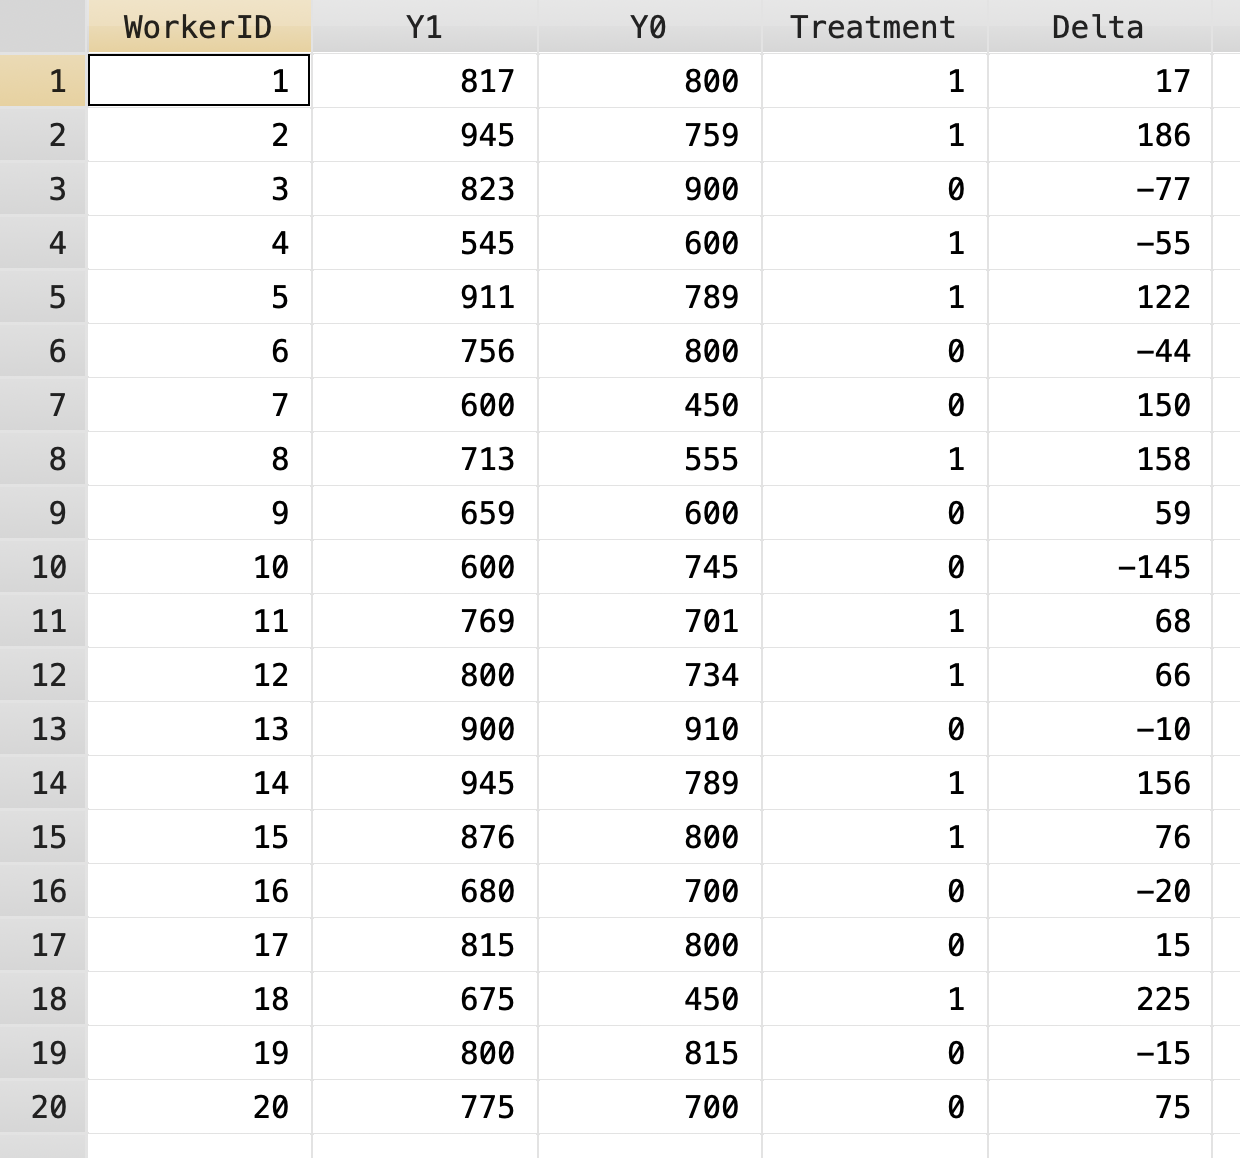
\includegraphics[keepaspectratio]{Week2_po_example.png}}
\caption{Potential Outcomes}
\end{figure}

The \(ATEU\) is -1.2.

\section{Calculate the ATE}\label{calculate-the-ate}

First we will calculate the average treatment effects \((ATE)\). We can calculate individual treatment effects under this hypothetical example and find the average treatment effects. What we calculate is \(ATE=E[Y^1]-E[Y^0]\)

We will find the mean for \(Y^1\) and the mean for \(Y^0\), and then subtract \(\mu_1\) from \(\mu_0\).

\begin{Shaded}
\begin{Highlighting}[]
\KeywordTok{egen}\NormalTok{ mean\_y1 = }\KeywordTok{mean}\NormalTok{(Y1)}
\KeywordTok{egen}\NormalTok{ mean\_y0 = }\KeywordTok{mean}\NormalTok{(Y0)}
\KeywordTok{gen}\NormalTok{ ate = mean\_y1 {-} mean\_y0}


\OtherTok{list}\NormalTok{ ate mean\_y1 mean\_y0 }\KeywordTok{in}\NormalTok{ 1/1}
\end{Highlighting}
\end{Shaded}

\begin{verbatim}
     |   ate   mean_y1   mean_y0 |
     |---------------------------|
  1. | 50.35     770.2    719.85 |
     +---------------------------+
\end{verbatim}

We estimate the average treatment effect to be 50.35.

\section{Calculate the ATET}\label{calculate-the-atet}

Next, we can calculate the average treatment effect on the treated \((ATET)\). We will subset only for those who actually received treatment. What we are calculating is \(ATET=E[Y^1|D=1]-E[Y^0|D=0]\).

\begin{Shaded}
\begin{Highlighting}[]
\KeywordTok{egen}\NormalTok{ mean\_y1\_d1 = }\KeywordTok{mean}\NormalTok{(Y1) }\KeywordTok{if}\NormalTok{ Treatment == 1}
\KeywordTok{egen}\NormalTok{ mean\_y0\_d1 = }\KeywordTok{mean}\NormalTok{(Y0) }\KeywordTok{if}\NormalTok{ Treatment == 1}
\KeywordTok{gen}\NormalTok{ att = mean\_y1\_d1 {-} mean\_y0\_d1}

\OtherTok{list}\NormalTok{ att mean\_y1\_d1 mean\_y0\_d1 }\KeywordTok{in}\NormalTok{ 1/1}
\end{Highlighting}
\end{Shaded}

\begin{verbatim}
(10 missing values generated)

(10 missing values generated)

(10 missing values generated)

     +-----------------------------+
     |   att   mea~1_d1   mea~0_d1 |
     |-----------------------------|
  1. | 101.9      799.6      697.7 |
     +-----------------------------+
\end{verbatim}

Our \(ATET\) is 101.9.

\section{Calculate the ATEU}\label{calculate-the-ateu}

Finally, we will estimate the average treatment effect on the untreated \((ATEU)\). We will subset for those who did not receive treatment. We are calculating \(ATEU=E[Y^1|D=0]-E[Y^0|D=0]\). In real life, we do not know \(E[Y^1|D=0]\)

\begin{Shaded}
\begin{Highlighting}[]
\KeywordTok{egen}\NormalTok{ mean\_y1\_d0 = }\KeywordTok{mean}\NormalTok{(Y1) }\KeywordTok{if}\NormalTok{ Treatment == 0}
\KeywordTok{egen}\NormalTok{ mean\_y0\_d0 = }\KeywordTok{mean}\NormalTok{(Y0) }\KeywordTok{if}\NormalTok{ Treatment == 0}
\KeywordTok{gen}\NormalTok{ atu = mean\_y1\_d0 {-} mean\_y0\_d0}

\OtherTok{list}\NormalTok{ atu mean\_y1\_d0 mean\_y0\_d0 }\KeywordTok{in}\NormalTok{ 3}
\end{Highlighting}
\end{Shaded}

\begin{verbatim}
(10 missing values generated)

(10 missing values generated)

(10 missing values generated)

     +----------------------------+
     |  atu   mea~1_d0   mea~0_d0 |
     |----------------------------|
  3. | -1.2      740.8        742 |
     +----------------------------+
\end{verbatim}

The \(ATEU\) is -1.6

\section{Calculate the SDO}\label{calculate-the-sdo}

We need to compare \(E[Y^1|D=1]\) and \(E[Y^0|D=0]\) to calculate the simple difference in outcomes. Since we have already calculated \(E[Y^1|D=1]\) and \(E[Y^0|D=0]\), we will just fill in the blanks with some Stata data managment.

First, we will set up a duplicate column for \(E[Y^1|D=1]\). Since we have a value for \(E[Y^1|D=1]\), we can push the value forward with \emph{{[}\_n-1{]}} or the prior value of the observation.

\begin{Shaded}
\begin{Highlighting}[]
\KeywordTok{gen}\NormalTok{ mean\_y1\_d1\_a = mean\_y1\_d1}
\KeywordTok{replace}\NormalTok{ mean\_y1\_d1\_a = mean\_y1\_d1\_a[}\DataTypeTok{\_n}\NormalTok{{-}1] }\KeywordTok{if} \FunctionTok{missing}\NormalTok{(mean\_y1\_d1\_a)}
\end{Highlighting}
\end{Shaded}

\begin{figure}
\centering
\pandocbounded{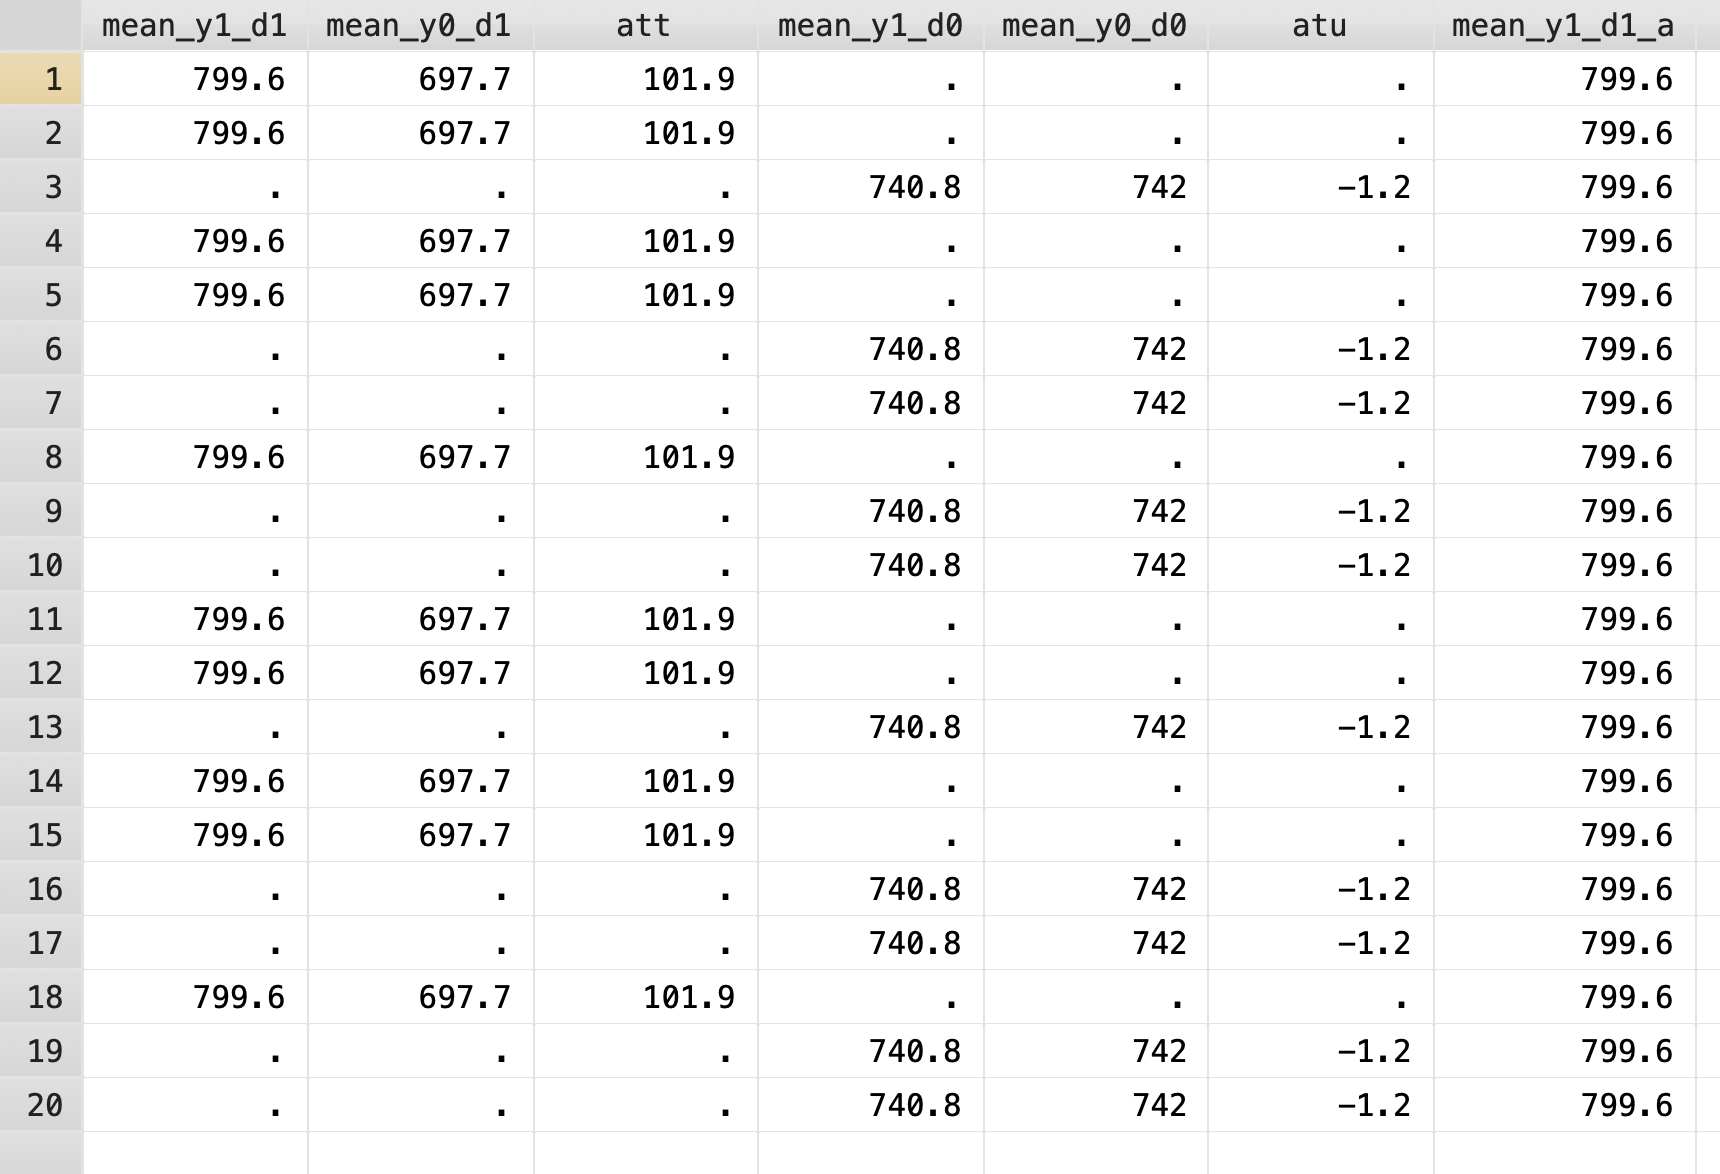
\includegraphics[keepaspectratio]{Week2_po_example2.png}}
\caption{Replace with lags}
\end{figure}

Next, we will set up a duplicate column for \(E[Y^0|D=0]\). Since we do not have a value for \(E[Y^0|D=0]\) in the first observation, we will need to add another line of code. We have \(E[Y^0|D=0]\) in the last value, so we can use {[}\_N{]} to get that observation and copy it to the first observation. Next, we will push the values forward similar to the prior example.

\begin{Shaded}
\begin{Highlighting}[]
\KeywordTok{gen}\NormalTok{ mean\_y0\_d0\_a = mean\_y0\_d0}

\KeywordTok{replace}\NormalTok{ mean\_y0\_d0\_a = mean\_y0\_d0\_a[\_N] }\KeywordTok{if} \FunctionTok{missing}\NormalTok{(mean\_y0\_d0\_a[1])}
\KeywordTok{replace}\NormalTok{ mean\_y0\_d0\_a = mean\_y0\_d0\_a[}\DataTypeTok{\_n}\NormalTok{{-}1] }\KeywordTok{if} \FunctionTok{missing}\NormalTok{(mean\_y0\_d0\_a)}
\end{Highlighting}
\end{Shaded}

\begin{figure}
\centering
\pandocbounded{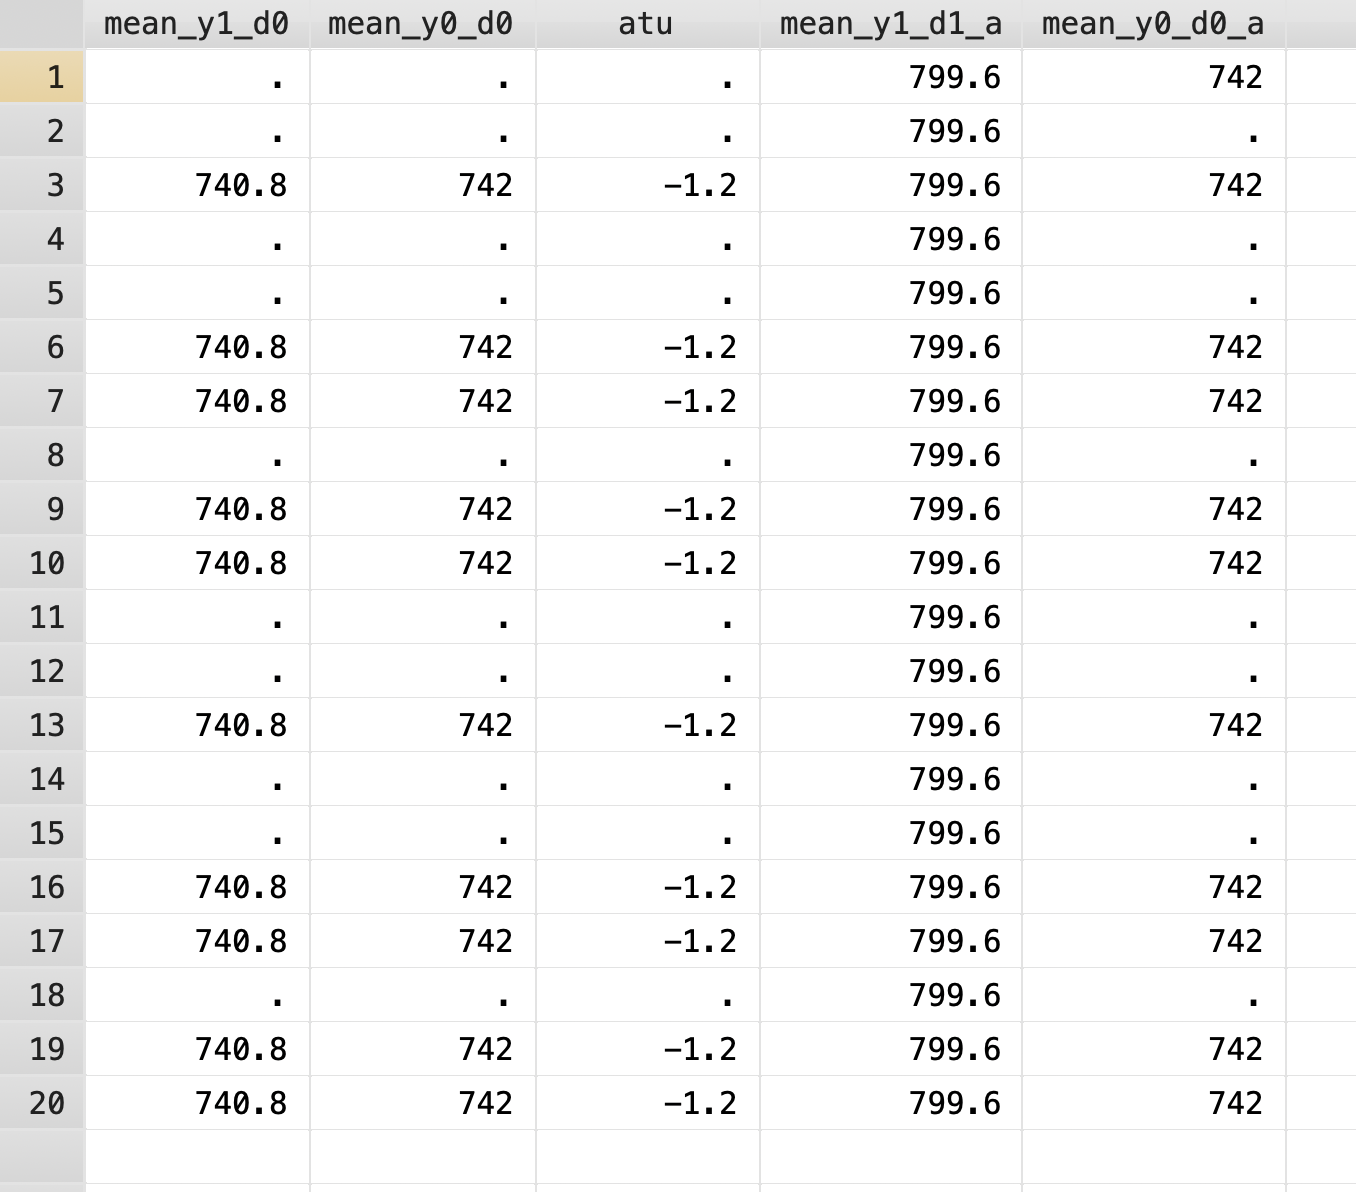
\includegraphics[keepaspectratio]{Week2_po_example3.png}}
\caption{Copy the Last observation to the first observation}
\end{figure}

Finally, we can calculate the simple difference in outcomes \((SDO)\).

\begin{Shaded}
\begin{Highlighting}[]
\KeywordTok{gen}\NormalTok{ sdo = .}
\KeywordTok{replace}\NormalTok{ sdo = mean\_y1\_d1\_a {-} mean\_y0\_d0\_a}
\OtherTok{list}\NormalTok{ ate sdo }\KeywordTok{if} \DataTypeTok{\_n}\NormalTok{ ==1}
\end{Highlighting}
\end{Shaded}

\begin{verbatim}
(20 missing values generated)

(20 real changes made)

     +--------------+
     |   ate    sdo |
     |--------------|
  1. | 50.35   57.6 |
     +--------------+
\end{verbatim}

The \(SDO\) is upwards biased by 6.25 dollars in this hypothetical example.

\chapter{Experimental Research Design}\label{experimental-research-design}

We can estimate the \(ATE\) using experimental research designs. If the experiments were well-designed and well-implemented experiments, then we can use the \emph{ttest} command to calculate the simple difference in outcomes or \(SDO\)

\section{Job Corps (2001) Evaluation}\label{job-corps-2001-evaluation}

The Deparment of Labor wanted an evaluation of the Job Corps program. The Job Corps program serves disadvantaged youth to improve employment outcomes. Individuals were randomly assigned to Job Corps or out of Job Corps due to limited slots.

\subsection{Inspect the Data}\label{inspect-the-data}

Let's inspect our outcome variable and treatment variable

\begin{Shaded}
\begin{Highlighting}[]
\NormalTok{cd }\StringTok{"/Users/Sam/Desktop/Econ 672/Data"}
\KeywordTok{use}\NormalTok{ JC, }\KeywordTok{clear}

\KeywordTok{describe}\NormalTok{ earny4}
\KeywordTok{describe}\NormalTok{ assignment}

\KeywordTok{sum}\NormalTok{ earny4}
\KeywordTok{tab}\NormalTok{ assignment}
\end{Highlighting}
\end{Shaded}

\begin{verbatim}
/Users/Sam/Desktop/Econ 672/Data

(Written by R.              )

              storage   display    value
variable name   type    format     label      variable label
----------------------------------------------------------------------------------------------------------------------
earny4          double  %9.0g                 Earnings 4 years after assignment

              storage   display    value
variable name   type    format     label      variable label
----------------------------------------------------------------------------------------------------------------------
assignment      double  %34.0g     assignment1
                                              Random assignment to Job Corps

              Earnings 4 years after assignment
-------------------------------------------------------------
      Percentiles      Smallest
 1%            0              0
 5%            0              0
10%            0              0       Obs               9,240
25%     43.50582              0       Sum of Wgt.       9,240

50%     181.7103                      Mean           207.6163
                        Largest       Std. Dev.      194.5507
75%     307.3206       1821.865
90%     442.1254       1859.233       Variance       37849.99
95%     544.7895       2357.738       Skewness       1.890325
99%     835.3426       2409.909       Kurtosis       12.32882

    Random assignment to Job Corps |      Freq.     Percent        Cum.
-----------------------------------+-----------------------------------
Randomly assigned out of Job Corps |      3,663       39.64       39.64
    Randomly assigned to Job Corps |      5,577       60.36      100.00
-----------------------------------+-----------------------------------
                             Total |      9,240      100.00
\end{verbatim}

Our outcome variable shows that the median earnings is \$181.71, while the mean is \$207.62.

Our treatment variable has 5,577 assigned to treatment and 3,663 assigned to the control group.

\subsection{Estimate the impact}\label{estimate-the-impact}

We can estimate the simple differnce in outcomes with the \emph{ttest} command.

\begin{Shaded}
\begin{Highlighting}[]
\KeywordTok{ttest}\NormalTok{ earny4, }\KeywordTok{by}\NormalTok{(assignment)}
\end{Highlighting}
\end{Shaded}

\begin{verbatim}
Two-sample t test with equal variances
------------------------------------------------------------------------------
   Group |     Obs        Mean    Std. Err.   Std. Dev.   [95% Conf. Interval]
---------+--------------------------------------------------------------------
Randomly |   3,663    197.9258    3.072182    185.9368    191.9025    203.9492
Randomly |   5,577     213.981    2.675004    199.7675    208.7369     219.225
---------+--------------------------------------------------------------------
combined |   9,240    207.6163    2.023936    194.5507    203.6489    211.5836
---------+--------------------------------------------------------------------
    diff |           -16.05513    4.134466               -24.15959   -7.950661
------------------------------------------------------------------------------
    diff = mean(Randomly) - mean(Randomly)                        t =  -3.8832
Ho: diff = 0                                     degrees of freedom =     9238

    Ha: diff < 0                 Ha: diff != 0                 Ha: diff > 0
 Pr(T < t) = 0.0001         Pr(|T| > |t|) = 0.0001          Pr(T > t) = 0.9999
\end{verbatim}

Next, let's run an OLS regression with and without robust standard errors

\begin{Shaded}
\begin{Highlighting}[]
\KeywordTok{reg}\NormalTok{ earny4 i.assignment}
\KeywordTok{reg}\NormalTok{ earny4 i.assignment, }\KeywordTok{robust}
\end{Highlighting}
\end{Shaded}

\begin{verbatim}
      Source |       SS           df       MS      Number of obs   =     9,240
-------------+----------------------------------   F(1, 9238)      =     15.08
       Model |  569892.708         1  569892.708   Prob > F        =    0.0001
    Residual |   349126136     9,238  37792.3941   R-squared       =    0.0016
-------------+----------------------------------   Adj R-squared   =    0.0015
       Total |   349696029     9,239  37849.9869   Root MSE        =     194.4

-------------------------------------------------------------------------------------------------
                         earny4 |      Coef.   Std. Err.      t    P>|t|     [95% Conf. Interval]
--------------------------------+----------------------------------------------------------------
                     assignment |
Randomly assigned to Job Corps  |   16.05513   4.134466     3.88   0.000     7.950661    24.15959
                          _cons |   197.9258   3.212061    61.62   0.000     191.6295    204.2222
-------------------------------------------------------------------------------------------------


Linear regression                               Number of obs     =      9,240
                                                F(1, 9238)        =      15.53
                                                Prob > F          =     0.0001
                                                R-squared         =     0.0016
                                                Root MSE          =      194.4

-------------------------------------------------------------------------------------------------
                                |               Robust
                         earny4 |      Coef.   Std. Err.      t    P>|t|     [95% Conf. Interval]
--------------------------------+----------------------------------------------------------------
                     assignment |
Randomly assigned to Job Corps  |   16.05513   4.073534     3.94   0.000     8.070101    24.04015
                          _cons |   197.9258   3.072095    64.43   0.000     191.9039    203.9478
-------------------------------------------------------------------------------------------------
\end{verbatim}

We see simple difference in outcomes is about 16 dollars higher, which is what we see in the Schochet, P. Z., Burghardt, J., Glazerman, S. (2001): ``National Job Corps study: The impacts of Job Corps on participants' employment and related outcomes'', Mathematica Policy Research, Washington, DC.

\subsection{Covariate Balance Test and Specification Tests}\label{covariate-balance-test-and-specification-tests}

Next, let's test the is there are any covariates associated with the treatment after randomization

\begin{Shaded}
\begin{Highlighting}[]

\KeywordTok{ttest}\NormalTok{ age, }\KeywordTok{by}\NormalTok{(assignment)}
\KeywordTok{ttest}\NormalTok{ educ, }\KeywordTok{by}\NormalTok{(assignment)}
\KeywordTok{ttest}\NormalTok{ educmum, }\KeywordTok{by}\NormalTok{(assignment)}
\KeywordTok{ttest}\NormalTok{ educdad, }\KeywordTok{by}\NormalTok{(assignment)}
\end{Highlighting}
\end{Shaded}

\begin{verbatim}
Two-sample t test with equal variances
------------------------------------------------------------------------------
   Group |     Obs        Mean    Std. Err.   Std. Dev.   [95% Conf. Interval]
---------+--------------------------------------------------------------------
Randomly |   3,663    18.33825     .034554    2.091302     18.2705    18.40599
Randomly |   5,577    18.50099    .0291468     2.17666    18.44385    18.55813
---------+--------------------------------------------------------------------
combined |   9,240    18.43647    .0223105    2.144592    18.39274    18.48021
---------+--------------------------------------------------------------------
    diff |           -.1627389    .0455812               -.2520881   -.0733896
------------------------------------------------------------------------------
    diff = mean(Randomly) - mean(Randomly)                        t =  -3.5703
Ho: diff = 0                                     degrees of freedom =     9238

    Ha: diff < 0                 Ha: diff != 0                 Ha: diff > 0
 Pr(T < t) = 0.0002         Pr(|T| > |t|) = 0.0004          Pr(T > t) = 0.9998


Two-sample t test with equal variances
------------------------------------------------------------------------------
   Group |     Obs        Mean    Std. Err.   Std. Dev.   [95% Conf. Interval]
---------+--------------------------------------------------------------------
Randomly |   3,663    9.924379    .0327304    1.980934    9.860207    9.988551
Randomly |   5,577    9.977228    .0270215    2.017948    9.924255     10.0302
---------+--------------------------------------------------------------------
combined |   9,240    9.956277    .0208418    2.003416    9.915423    9.997132
---------+--------------------------------------------------------------------
    diff |            -.052849    .0426065               -.1363671    .0306691
------------------------------------------------------------------------------
    diff = mean(Randomly) - mean(Randomly)                        t =  -1.2404
Ho: diff = 0                                     degrees of freedom =     9238

    Ha: diff < 0                 Ha: diff != 0                 Ha: diff > 0
 Pr(T < t) = 0.1074         Pr(|T| > |t|) = 0.2149          Pr(T > t) = 0.8926


Two-sample t test with equal variances
------------------------------------------------------------------------------
   Group |     Obs        Mean    Std. Err.   Std. Dev.   [95% Conf. Interval]
---------+--------------------------------------------------------------------
Randomly |   3,663    9.280917     .084987    5.143648    9.114291    9.447544
Randomly |   5,577    9.335664    .0675206    5.042389    9.203298    9.468031
---------+--------------------------------------------------------------------
combined |   9,240    9.313961    .0528746    5.082565    9.210315    9.417607
---------+--------------------------------------------------------------------
    diff |           -.0547471     .108098                -.266643    .1571489
------------------------------------------------------------------------------
    diff = mean(Randomly) - mean(Randomly)                        t =  -0.5065
Ho: diff = 0                                     degrees of freedom =     9238

    Ha: diff < 0                 Ha: diff != 0                 Ha: diff > 0
 Pr(T < t) = 0.3063         Pr(|T| > |t|) = 0.6125          Pr(T > t) = 0.6937


Two-sample t test with equal variances
------------------------------------------------------------------------------
   Group |     Obs        Mean    Std. Err.   Std. Dev.   [95% Conf. Interval]
---------+--------------------------------------------------------------------
Randomly |   3,663    7.019383    .1004599    6.080105     6.82242    7.216346
Randomly |   5,577     7.04662    .0803195    5.998205    6.889163    7.204078
---------+--------------------------------------------------------------------
combined |   9,240    7.035823     .062736    6.030492    6.912846    7.158799
---------+--------------------------------------------------------------------
    diff |            -.027237    .1282603               -.2786556    .2241816
------------------------------------------------------------------------------
    diff = mean(Randomly) - mean(Randomly)                        t =  -0.2124
Ho: diff = 0                                     degrees of freedom =     9238

    Ha: diff < 0                 Ha: diff != 0                 Ha: diff > 0
 Pr(T < t) = 0.4159         Pr(|T| > |t|) = 0.8318          Pr(T > t) = 0.5841
\end{verbatim}

We fail to reject the null hypothesis that there are differences between treatment and control among the covariates of age, education attained, mother's education, and father's education.

\begin{Shaded}
\begin{Highlighting}[]
\KeywordTok{tab} \BaseNTok{black}\NormalTok{ assignment, }\FunctionTok{chi2}
\KeywordTok{tab}\NormalTok{ female assignment, }\FunctionTok{chi2}
\KeywordTok{tab}\NormalTok{ hispanic assignment, }\FunctionTok{chi2}
\KeywordTok{tab}\NormalTok{ cohabmarried assignment, }\FunctionTok{chi2}
\KeywordTok{tab}\NormalTok{ haschild assignment, }\FunctionTok{chi2}
\end{Highlighting}
\end{Shaded}

\begin{verbatim}
Individual |
  is Black | Random assignment to
or African |       Job Corps
  American | Randomly   Randomly  |     Total
-----------+----------------------+----------
 Non-Black |     1,873      2,810 |     4,683 
     Black |     1,790      2,767 |     4,557 
-----------+----------------------+----------
     Total |     3,663      5,577 |     9,240 

          Pearson chi2(1) =   0.4941   Pr = 0.482

           | Random assignment to
Individual |       Job Corps
 is female | Randomly   Randomly  |     Total
-----------+----------------------+----------
      Male |     2,220      2,960 |     5,180 
    Female |     1,443      2,617 |     4,060 
-----------+----------------------+----------
     Total |     3,663      5,577 |     9,240 

          Pearson chi2(1) =  50.9039   Pr = 0.000

                | Random assignment to
  Individual is |       Job Corps
Latino/Hispanic | Randomly   Randomly  |     Total
----------------+----------------------+----------
     Non-Latino |     3,024      4,641 |     7,665 
Latino/Hispanic |       639        936 |     1,575 
----------------+----------------------+----------
          Total |     3,663      5,577 |     9,240 

          Pearson chi2(1) =   0.6842   Pr = 0.408


Individual is Married | Random assignment to
     or Cohabiting at |       Job Corps
           assignment | Randomly   Randomly  |     Total
----------------------+----------------------+----------
Not Married or cohabi |     3,441      5,233 |     8,674 
Married or Cohabiting |       222        344 |       566 
----------------------+----------------------+----------
                Total |     3,663      5,577 |     9,240 

          Pearson chi2(1) =   0.0445   Pr = 0.833


 Individual has child | Random assignment to
       or children at |       Job Corps
           assignment | Randomly   Randomly  |     Total
----------------------+----------------------+----------
           No chilren |     2,981      4,417 |     7,398 
Has at least one chil |       682      1,160 |     1,842 
----------------------+----------------------+----------
                Total |     3,663      5,577 |     9,240 

          Pearson chi2(1) =   6.5895   Pr = 0.010


  Individual |
    has ever | Random assignment to
   worked at |       Job Corps
  assignment | Randomly   Randomly  |     Total
-------------+----------------------+----------
Never worked |     3,155      4,767 |     7,922 
  Has worked |       508        810 |     1,318 
-------------+----------------------+----------
       Total |     3,663      5,577 |     9,240 

          Pearson chi2(1) =   0.7768   Pr = 0.378
\end{verbatim}

We see that we fail to reject the null hypothesis that there is a difference between treatment and control for individuals for Black, Latino/Hispanic, Married/Cohabiting, and Ever Worked. However, we reject the null hypothesis that there is no difference between treatment and control for being female or having any children.

Should we be concerned? Yes!

Let's do a sensitivity tests. The first model will be the simple difference, while the second model will include the covariates we rejected the null hypothesis. The third model will include all covariates.

While there is some concern for a lack of covariate balance, the full data set utilizes weights which we do not have in the public use data.

*What happens to the standard errors

\begin{Shaded}
\begin{Highlighting}[]
\KeywordTok{est} \KeywordTok{clear}
\NormalTok{eststo m1: }\KeywordTok{quietly} \KeywordTok{reg}\NormalTok{ earny4 i.assignment}
\NormalTok{eststo m2: }\KeywordTok{quietly} \KeywordTok{reg}\NormalTok{ earny4 i.assignment i.female i.haschild}
\NormalTok{eststo m3: }\KeywordTok{quietly} \KeywordTok{reg}\NormalTok{ earny4 i.assignment i.female i.}\BaseNTok{black}\NormalTok{ i.hispanic i.cohabmarried i.haschild i.everwkd age educ educmum educdad}

\NormalTok{esttab m1 m2 m3, mtitle(}\StringTok{"Model 1"} \StringTok{"Model 2"} \StringTok{"Model 3"}\NormalTok{) }\KeywordTok{keep}\NormalTok{(1.assignment)}
\end{Highlighting}
\end{Shaded}

\begin{verbatim}
                      (1)             (2)             (3)   
                  Model 1         Model 2         Model 3   
------------------------------------------------------------
1.assignment        16.06***        21.07***        19.59***
                   (3.88)          (5.16)          (4.96)   
------------------------------------------------------------
N                    9240            9240            9240   
------------------------------------------------------------
t statistics in parentheses
* p<0.05, ** p<0.01, *** p<0.001
\end{verbatim}

We see that our ATE increase estimates range from 16 dollars to 21 dollars.

\section{Leaftlet Information Evaluation}\label{leaftlet-information-evaluation}

Next we will look at an impact evaluation of an information leaflet about coffee production on students' awareness. The target population is Bulgarian high school and high school students and the outcome is the awareness of environmental issues due to coffee production.

\subsection{Inspect the Data}\label{inspect-the-data-1}

Let's inspect the data by running some descriptive statistics. Our dependent variable is awarewaste, while treatment is a leaflet treatment is randomly assigned to students.

\begin{Shaded}
\begin{Highlighting}[]
\NormalTok{cd }\StringTok{"/Users/Sam/Desktop/Econ 672/Data"}
\KeywordTok{use}\NormalTok{ CoffeeLeaflet, }\KeywordTok{clear}

\KeywordTok{tab}\NormalTok{ awarewaste}
\KeywordTok{tab}\NormalTok{ treatment}
\end{Highlighting}
\end{Shaded}

\begin{verbatim}
/Users/Sam/Desktop/Econ 672/Data

(Written by R.              )








Awareness of waste |
 production due to |
 coffee production |      Freq.     Percent        Cum.
-------------------+-----------------------------------
         Not Aware |        171       33.93       33.93
Slightly Not Aware |        157       31.15       65.08
           Neither |        121       24.01       89.09
    Slightly Aware |         41        8.13       97.22
       Fully Aware |         14        2.78      100.00
-------------------+-----------------------------------
             Total |        504      100.00

       Treatment Status |      Freq.     Percent        Cum.
------------------------+-----------------------------------
          Control Group |        261       50.00       50.00
Leaflet Treatment Group |        261       50.00      100.00
------------------------+-----------------------------------
                  Total |        522      100.00
\end{verbatim}

\subsection{Estimate the impact}\label{estimate-the-impact-1}

Let's run the simple difference in outcomes with \emph{ttest} command.

\begin{Shaded}
\begin{Highlighting}[]
\KeywordTok{ttest}\NormalTok{ awarewaste, }\KeywordTok{by}\NormalTok{(treatment)}
\end{Highlighting}
\end{Shaded}

\begin{verbatim}
Two-sample t test with equal variances
------------------------------------------------------------------------------
   Group |     Obs        Mean    Std. Err.   Std. Dev.   [95% Conf. Interval]
---------+--------------------------------------------------------------------
 Control |     254    2.007874    .0628675    1.001943    1.884064    2.131684
 Leaflet |     250       2.288    .0702564    1.110852    2.149627    2.426373
---------+--------------------------------------------------------------------
combined |     504    2.146825    .0474646    1.065578    2.053572    2.240079
---------+--------------------------------------------------------------------
    diff |            -.280126    .0942007               -.4652021   -.0950498
------------------------------------------------------------------------------
    diff = mean(Control) - mean(Leaflet)                          t =  -2.9737
Ho: diff = 0                                     degrees of freedom =      502

    Ha: diff < 0                 Ha: diff != 0                 Ha: diff > 0
 Pr(T < t) = 0.0015         Pr(|T| > |t|) = 0.0031          Pr(T > t) = 0.9985
\end{verbatim}

We reject the null hypothesis that the leaflet treatment had no impact, and it increases awareness by 0.28.

Let's run an OLS regression.

\begin{Shaded}
\begin{Highlighting}[]
\KeywordTok{reg}\NormalTok{ awarewaste i.treatment}
\end{Highlighting}
\end{Shaded}

\begin{verbatim}
      Source |       SS           df       MS      Number of obs   =       504
-------------+----------------------------------   F(1, 502)       =      8.84
       Model |  9.88666867         1  9.88666867   Prob > F        =    0.0031
    Residual |  561.248252       502  1.11802441   R-squared       =    0.0173
-------------+----------------------------------   Adj R-squared   =    0.0154
       Total |  571.134921       503   1.1354571   Root MSE        =    1.0574

------------------------------------------------------------------------------------------
              awarewaste |      Coef.   Std. Err.      t    P>|t|     [95% Conf. Interval]
-------------------------+----------------------------------------------------------------
               treatment |
Leaflet Treatment Group  |    .280126   .0942007     2.97   0.003     .0950498    .4652021
                   _cons |   2.007874   .0663451    30.26   0.000     1.877526    2.138222
------------------------------------------------------------------------------------------
\end{verbatim}

Wait a second! What does 0.28 mean? What is a potential problem here?

Look at the outcome variable again. It is an ordinal variable! Let's use a \(\chi^2\) test

\begin{Shaded}
\begin{Highlighting}[]
\KeywordTok{tab}\NormalTok{ awarewaste treatment, }\FunctionTok{chi2}
\end{Highlighting}
\end{Shaded}

\begin{verbatim}
Awareness of waste |
 production due to |   Treatment Status
 coffee production | Control G  Leaflet T |     Total
-------------------+----------------------+----------
         Not Aware |        97         74 |       171 
Slightly Not Aware |        82         75 |       157 
           Neither |        56         65 |       121 
    Slightly Aware |        14         27 |        41 
       Fully Aware |         5          9 |        14 
-------------------+----------------------+----------
             Total |       254        250 |       504 

          Pearson chi2(4) =   9.3087   Pr = 0.054
\end{verbatim}

Let's run an ordinal logit regression.

\begin{Shaded}
\begin{Highlighting}[]
\KeywordTok{ologit}\NormalTok{ awarewaste i.treatment, }\KeywordTok{or}
\end{Highlighting}
\end{Shaded}

\begin{verbatim}
Iteration 0:   log likelihood = -693.62947  
Iteration 1:   log likelihood = -689.57824  
Iteration 2:   log likelihood = -689.57505  
Iteration 3:   log likelihood = -689.57505  

Ordered logistic regression                     Number of obs     =        504
                                                LR chi2(1)        =       8.11
                                                Prob > chi2       =     0.0044
Log likelihood = -689.57505                     Pseudo R2         =     0.0058

------------------------------------------------------------------------------------------
              awarewaste |      Coef.   Std. Err.      z    P>|z|     [95% Conf. Interval]
-------------------------+----------------------------------------------------------------
               treatment |
Leaflet Treatment Group  |   .4609564   .1623425     2.84   0.005     .1427709    .7791419
-------------------------+----------------------------------------------------------------
                   /cut1 |  -.4493223   .1211244                     -.6867218   -.2119229
                   /cut2 |   .8543491   .1252889                      .6087873    1.099911
                   /cut3 |   2.346133    .168949                      2.014999    2.677267
                   /cut4 |    3.80845   .2865533                      3.246816    4.370084
------------------------------------------------------------------------------------------
\end{verbatim}

Individuals who received treatment were 1.46 times more likely to be aware of the effect of coffee production on environmental issues than those in the control group.

\subsection{Covariate Balance Test}\label{covariate-balance-test}

Let's test covariate balance

\begin{Shaded}
\begin{Highlighting}[]
\KeywordTok{foreach}\NormalTok{ v }\KeywordTok{of} \KeywordTok{varlist}\NormalTok{ sex mumedu dadedu bulgnationality drinkcoffee citysofia \{}
  \KeywordTok{tab}\NormalTok{ awarewaste }\OtherTok{\textasciigrave{}v\textquotesingle{}}\NormalTok{, }\FunctionTok{chi2}
\NormalTok{\}}
\end{Highlighting}
\end{Shaded}

\begin{verbatim}
Awareness of waste |
 production due to |          sex
 coffee production |         0          1 |     Total
-------------------+----------------------+----------
         Not Aware |        94         77 |       171 
Slightly Not Aware |       102         53 |       155 
           Neither |        65         55 |       120 
    Slightly Aware |        22         19 |        41 
       Fully Aware |         3         11 |        14 
-------------------+----------------------+----------
             Total |       286        215 |       501 

          Pearson chi2(4) =  13.0039   Pr = 0.011

Awareness of waste |
 production due to |              mumedu
 coffee production |         1          2          3 |     Total
-------------------+---------------------------------+----------
         Not Aware |         3         69         88 |       160 
Slightly Not Aware |         5         48         98 |       151 
           Neither |         1         31         76 |       108 
    Slightly Aware |         1          9         27 |        37 
       Fully Aware |         0          3          9 |        12 
-------------------+---------------------------------+----------
             Total |        10        160        298 |       468 

          Pearson chi2(8) =  11.8017   Pr = 0.160

Awareness of waste |
 production due to |              dadedu
 coffee production |         1          2          3 |     Total
-------------------+---------------------------------+----------
         Not Aware |         4         67         83 |       154 
Slightly Not Aware |         2         53         87 |       142 
           Neither |         0         42         62 |       104 
    Slightly Aware |         0          9         30 |        39 
       Fully Aware |         0          3          8 |        11 
-------------------+---------------------------------+----------
             Total |         6        174        270 |       450 

          Pearson chi2(8) =  10.9594   Pr = 0.204

Awareness of waste |
 production due to |    bulgnationality
 coffee production |         0          1 |     Total
-------------------+----------------------+----------
         Not Aware |         4        167 |       171 
Slightly Not Aware |         5        152 |       157 
           Neither |         2        119 |       121 
    Slightly Aware |         0         41 |        41 
       Fully Aware |         0         14 |        14 
-------------------+----------------------+----------
             Total |        11        493 |       504 

          Pearson chi2(4) =   2.1444   Pr = 0.709

Awareness of waste |
 production due to |                      drinkcoffee
 coffee production |         1          2          3          4          5 |     Total
-------------------+-------------------------------------------------------+----------
         Not Aware |        68         18         21         32         31 |       170 
Slightly Not Aware |        39         25         32         27         34 |       157 
           Neither |        46         19         19         21         14 |       119 
    Slightly Aware |        12          5          4         12          8 |        41 
       Fully Aware |         4          0          4          3          2 |        13 
-------------------+-------------------------------------------------------+----------
             Total |       169         67         80         95         89 |       500 

         Pearson chi2(16) =  23.6155   Pr = 0.098

Awareness of waste |
 production due to |       citysofia
 coffee production |         0          1 |     Total
-------------------+----------------------+----------
         Not Aware |        46        125 |       171 
Slightly Not Aware |        40        117 |       157 
           Neither |        27         94 |       121 
    Slightly Aware |         7         34 |        41 
       Fully Aware |         2         12 |        14 
-------------------+----------------------+----------
             Total |       122        382 |       504 

          Pearson chi2(4) =   2.9391   Pr = 0.568
\end{verbatim}

From our covariate balance test, we have a slight concern for imbalance in sex. However, all other characteristics were no correlated with treatment status.

\begin{Shaded}
\begin{Highlighting}[]
\KeywordTok{est} \KeywordTok{clear}
\KeywordTok{quietly}\NormalTok{ \{}
\NormalTok{eststo m1: }\KeywordTok{ologit}\NormalTok{ awarewaste i.treatment, }\KeywordTok{or}
\NormalTok{eststo m2: }\KeywordTok{ologit}\NormalTok{ awarewaste i.treatment i.mumedu i.sex, }\KeywordTok{or}
\NormalTok{eststo m3: }\KeywordTok{ologit}\NormalTok{ awarewaste i.treatment i.drinkcoffee i.sex i.mumedu i.dadedu i.bulgnationality i.citysofia, }\KeywordTok{or}
\NormalTok{\}}

\NormalTok{esttab m1 m2 m3, mtitle(}\StringTok{"Model 1"} \StringTok{"Model 2"} \StringTok{"Model 3"}\NormalTok{) }\KeywordTok{keep}\NormalTok{(1.treatment)}
\end{Highlighting}
\end{Shaded}

\begin{verbatim}
                      (1)             (2)             (3)   
                  Model 1         Model 2         Model 3   
------------------------------------------------------------
awarewaste                                                  
1.treatment         0.461**         0.566***        0.583** 
                   (2.84)          (3.32)          (3.27)   
------------------------------------------------------------
N                     504             466             434   
------------------------------------------------------------
t statistics in parentheses
* p<0.05, ** p<0.01, *** p<0.001
\end{verbatim}

Our estimates range from an odd ratio of 1.46 to 1.58. Notice that as we add covariates, our sample size is dropping, which means not all observations provided characteristic information.

\chapter{Randomized Inference}\label{randomized-inference}

Adapted from Cunningham (2021)

We will use a placebo-based test to calculate exact p-values. We need every single permutation of treatment to calculate the exact p-values from the ATE.

\section{Set up the Dataset}\label{set-up-the-dataset}

First we will set the seed so we can replicate our randomized results

\begin{Shaded}
\begin{Highlighting}[]
\KeywordTok{set} \DecValTok{seed}\NormalTok{ 1234}
\end{Highlighting}
\end{Shaded}

Next we will bring in our

\begin{Shaded}
\begin{Highlighting}[]
\NormalTok{cd }\StringTok{"/Users/Sam/Desktop/Econ 672/Data"}
\KeywordTok{use}\NormalTok{ ri.dta, }\KeywordTok{clear}
\KeywordTok{tempfile}\NormalTok{ ri}
\KeywordTok{gen}\NormalTok{ id = }\DataTypeTok{\_n}
\KeywordTok{save} \StringTok{"\textasciigrave{}ri\textquotesingle{}"}\NormalTok{, }\KeywordTok{replace}
\end{Highlighting}
\end{Shaded}

\pandocbounded{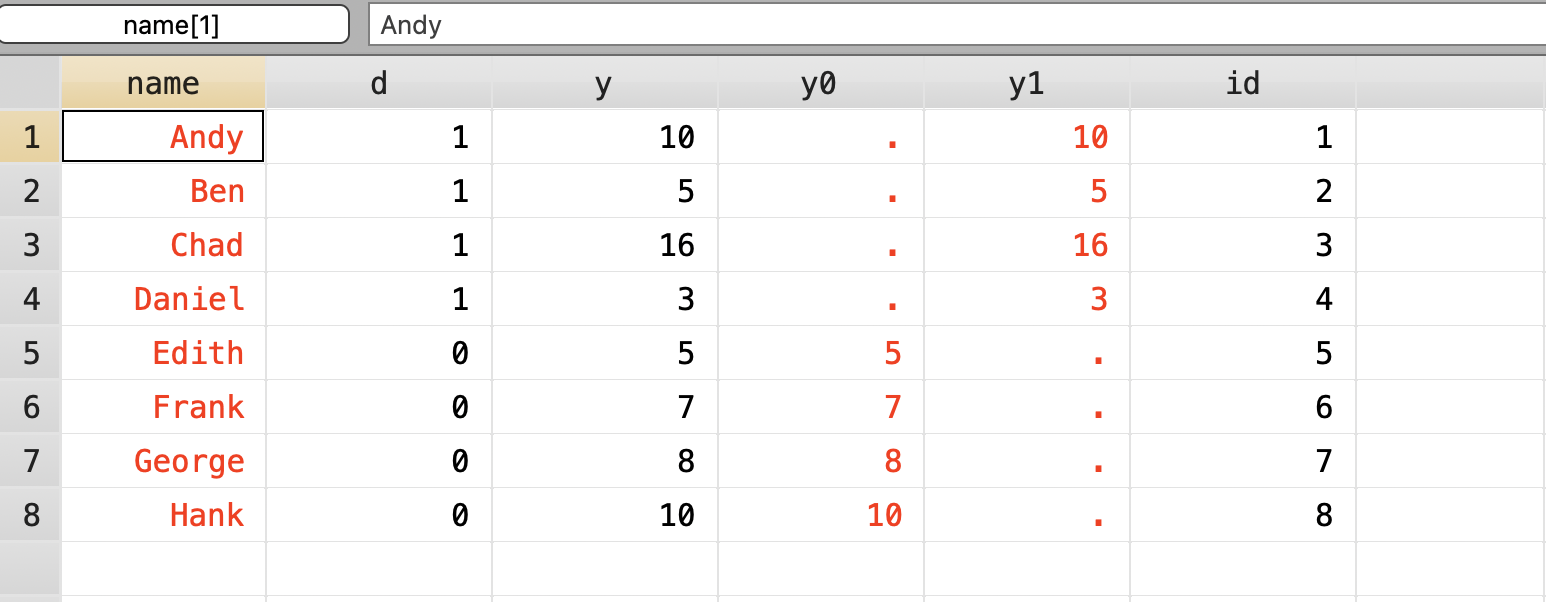
\includegraphics[keepaspectratio]{Week2_ri_example.png}}
Next we will create all combinations from our eight observations. We will need to install the \emph{percom} package into stata.

\begin{Shaded}
\begin{Highlighting}[]
\KeywordTok{ssc}\NormalTok{ install percom}
\end{Highlighting}
\end{Shaded}

Out of 8 observations, we get 70 permutations.
We can use the \emph{combin} command to get these permutations. From the \emph{help combin}, the \emph{combin} command generates \(k\) unique combinations from a set of \(n\) objects, where \(k\) is not greater than \(5 (2 =< k <= 5)\).
Program first arranges \(k\) possible permutations and then retains unique combinations. It supports both string and numeric variables.

combination: \(\frac{n!}{k!(n-k)!}\)

We will tell the \emph{combin} command that we want 4 combinations from our 8 observations.

\begin{Shaded}
\begin{Highlighting}[]
\NormalTok{combin id, }\KeywordTok{k}\NormalTok{(4)}
\end{Highlighting}
\end{Shaded}

\begin{verbatim}
         k =          4
         N =          8
Combinations Formed: 70
\end{verbatim}

\pandocbounded{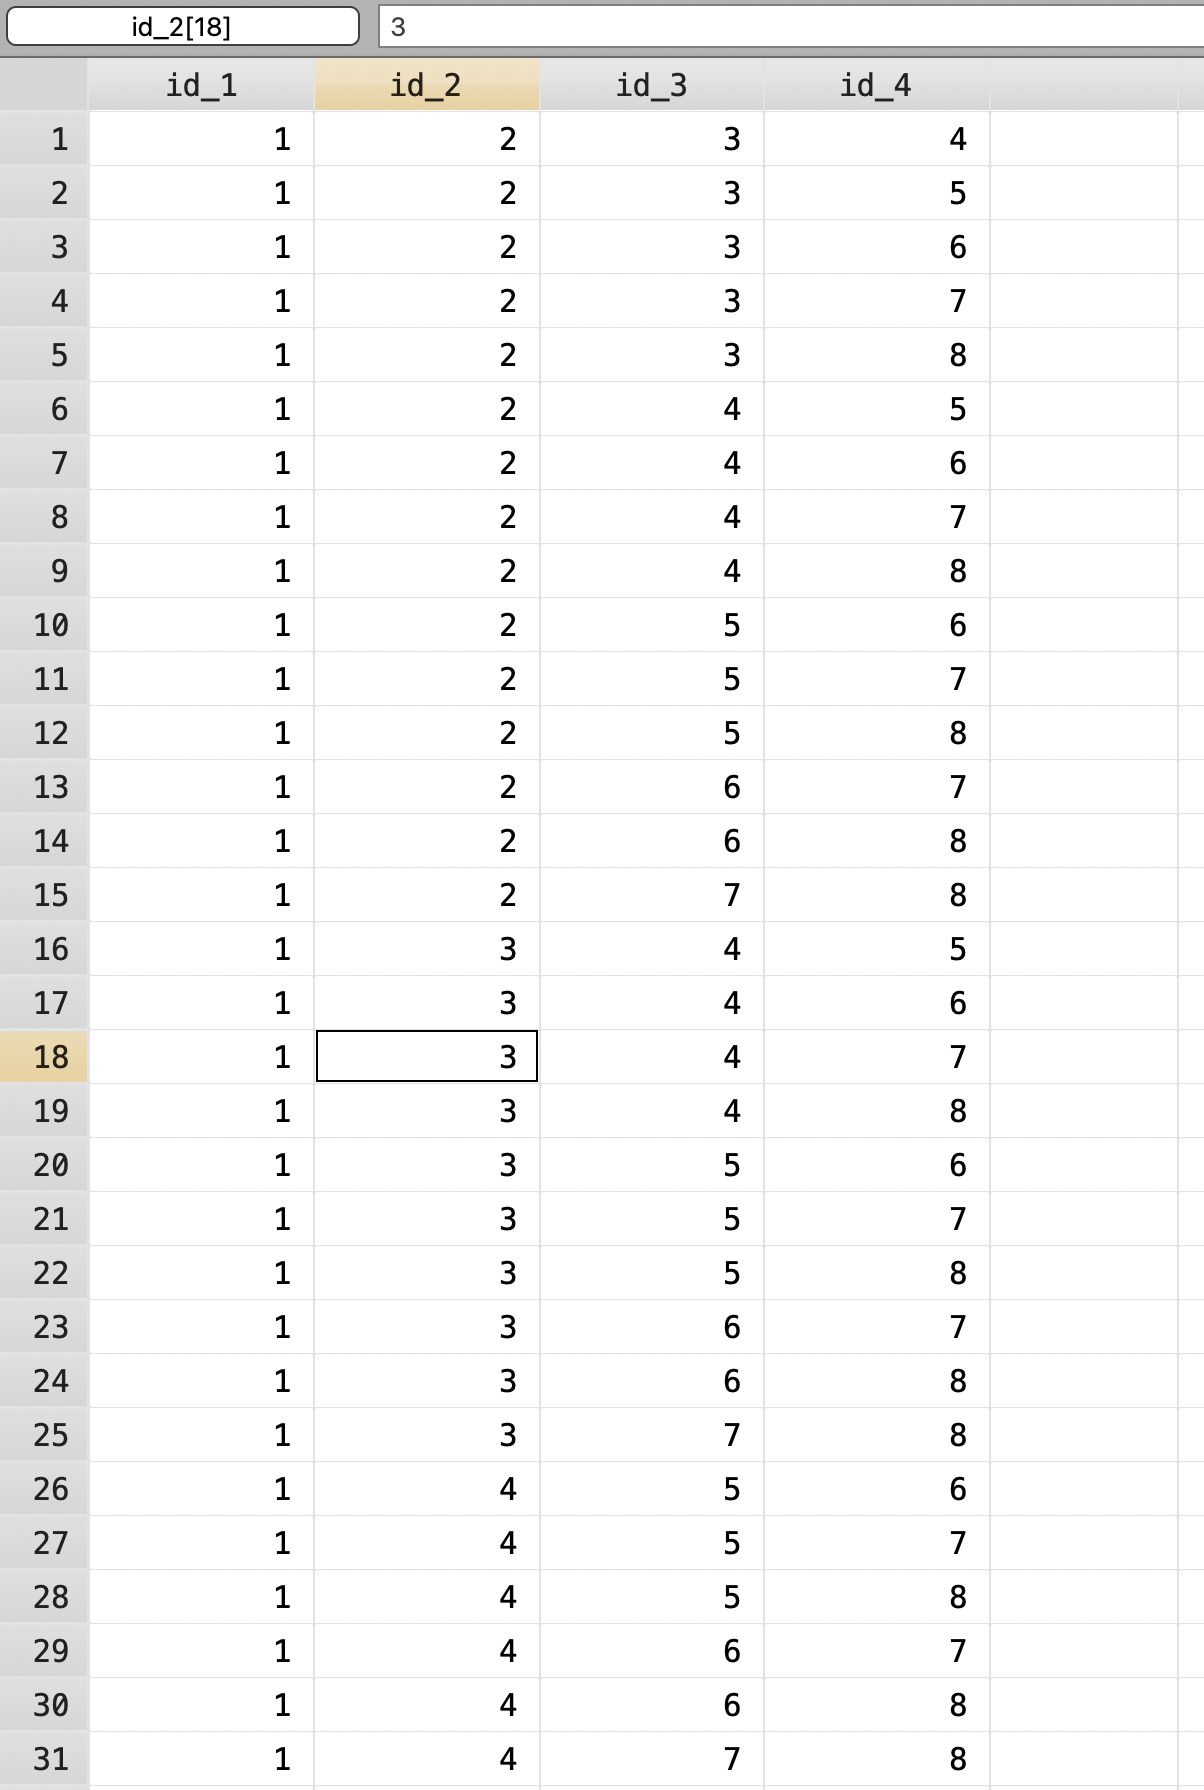
\includegraphics[keepaspectratio]{Week2_ri_example2.png}}
Next we will label the permutations 1 to 70.

\begin{Shaded}
\begin{Highlighting}[]
\KeywordTok{gen}\NormalTok{ permutation = }\DataTypeTok{\_n}
\KeywordTok{tempfile}\NormalTok{ combo}
\KeywordTok{save} \StringTok{"\textasciigrave{}combo\textquotesingle{}"}\NormalTok{, }\KeywordTok{replace}

\NormalTok{forvalue i =1/4 \{}
    \KeywordTok{rename}\NormalTok{ id\_}\OtherTok{\textasciigrave{}i\textquotesingle{}}\NormalTok{ treated}\OtherTok{\textasciigrave{}i\textquotesingle{}}
\NormalTok{\}}
\end{Highlighting}
\end{Shaded}

Next we will merge our permutations with our dataset of potential outcomes

\begin{Shaded}
\begin{Highlighting}[]
\KeywordTok{destring}\NormalTok{ treated*, }\KeywordTok{replace}
\KeywordTok{cross} \KeywordTok{using} \OtherTok{\textasciigrave{}ri\textquotesingle{}}
\end{Highlighting}
\end{Shaded}

\begin{figure}
\centering
\pandocbounded{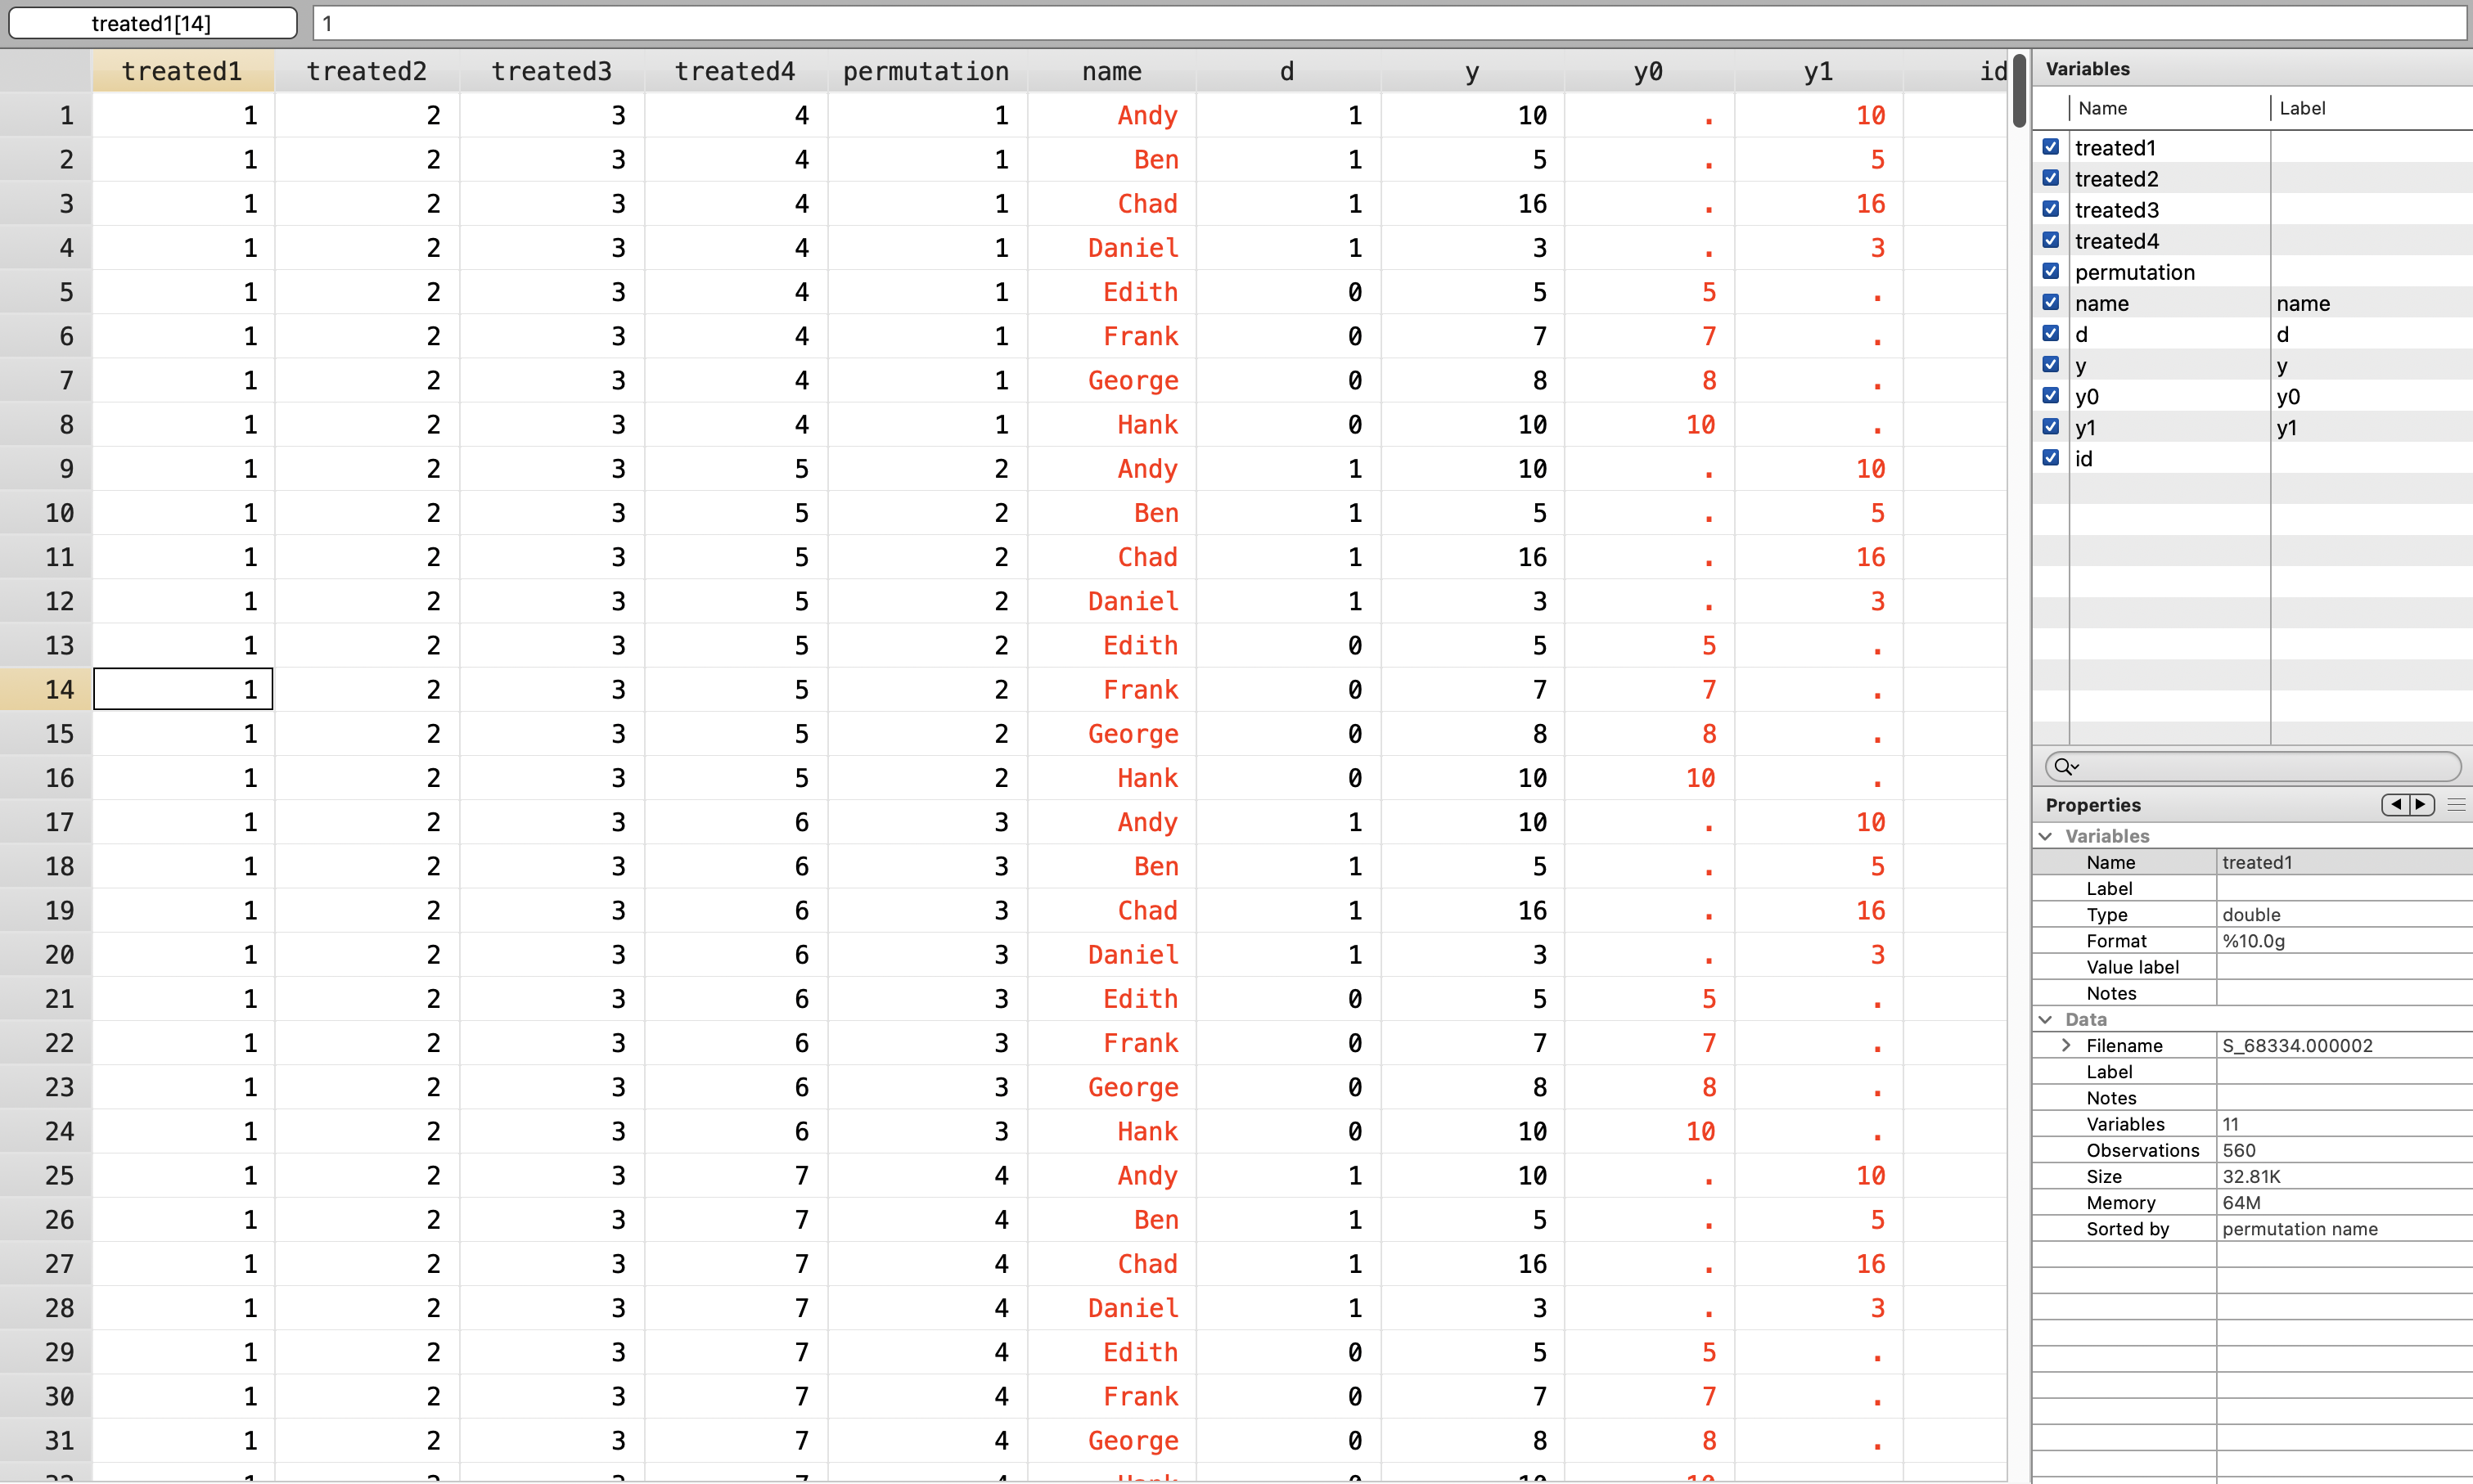
\includegraphics[keepaspectratio]{Week2_ri_example3.png}}
\caption{Merge Dataset with Permutations}
\end{figure}

\section{Randomize Assignment to Treatment}\label{randomize-assignment-to-treatment}

Next we will randomized treatment and calculate other test statistics.

First, we create a fake treatment variable \(d2\)

\begin{Shaded}
\begin{Highlighting}[]
\KeywordTok{gen}\NormalTok{ d2 = .}
\KeywordTok{replace}\NormalTok{ d2 = 1 }\KeywordTok{if}\NormalTok{ id == treated1 | id == treated2 | id == treated3 | id == treated4}
\KeywordTok{replace}\NormalTok{ d2 = 0 }\KeywordTok{if}\NormalTok{ \textasciitilde{}(id == treated1 | id == treated2 | id == treated3 | id == treated4)}
\KeywordTok{gen}\NormalTok{ check = }\KeywordTok{d}\NormalTok{ {-} d2}
\end{Highlighting}
\end{Shaded}

\begin{figure}
\centering
\pandocbounded{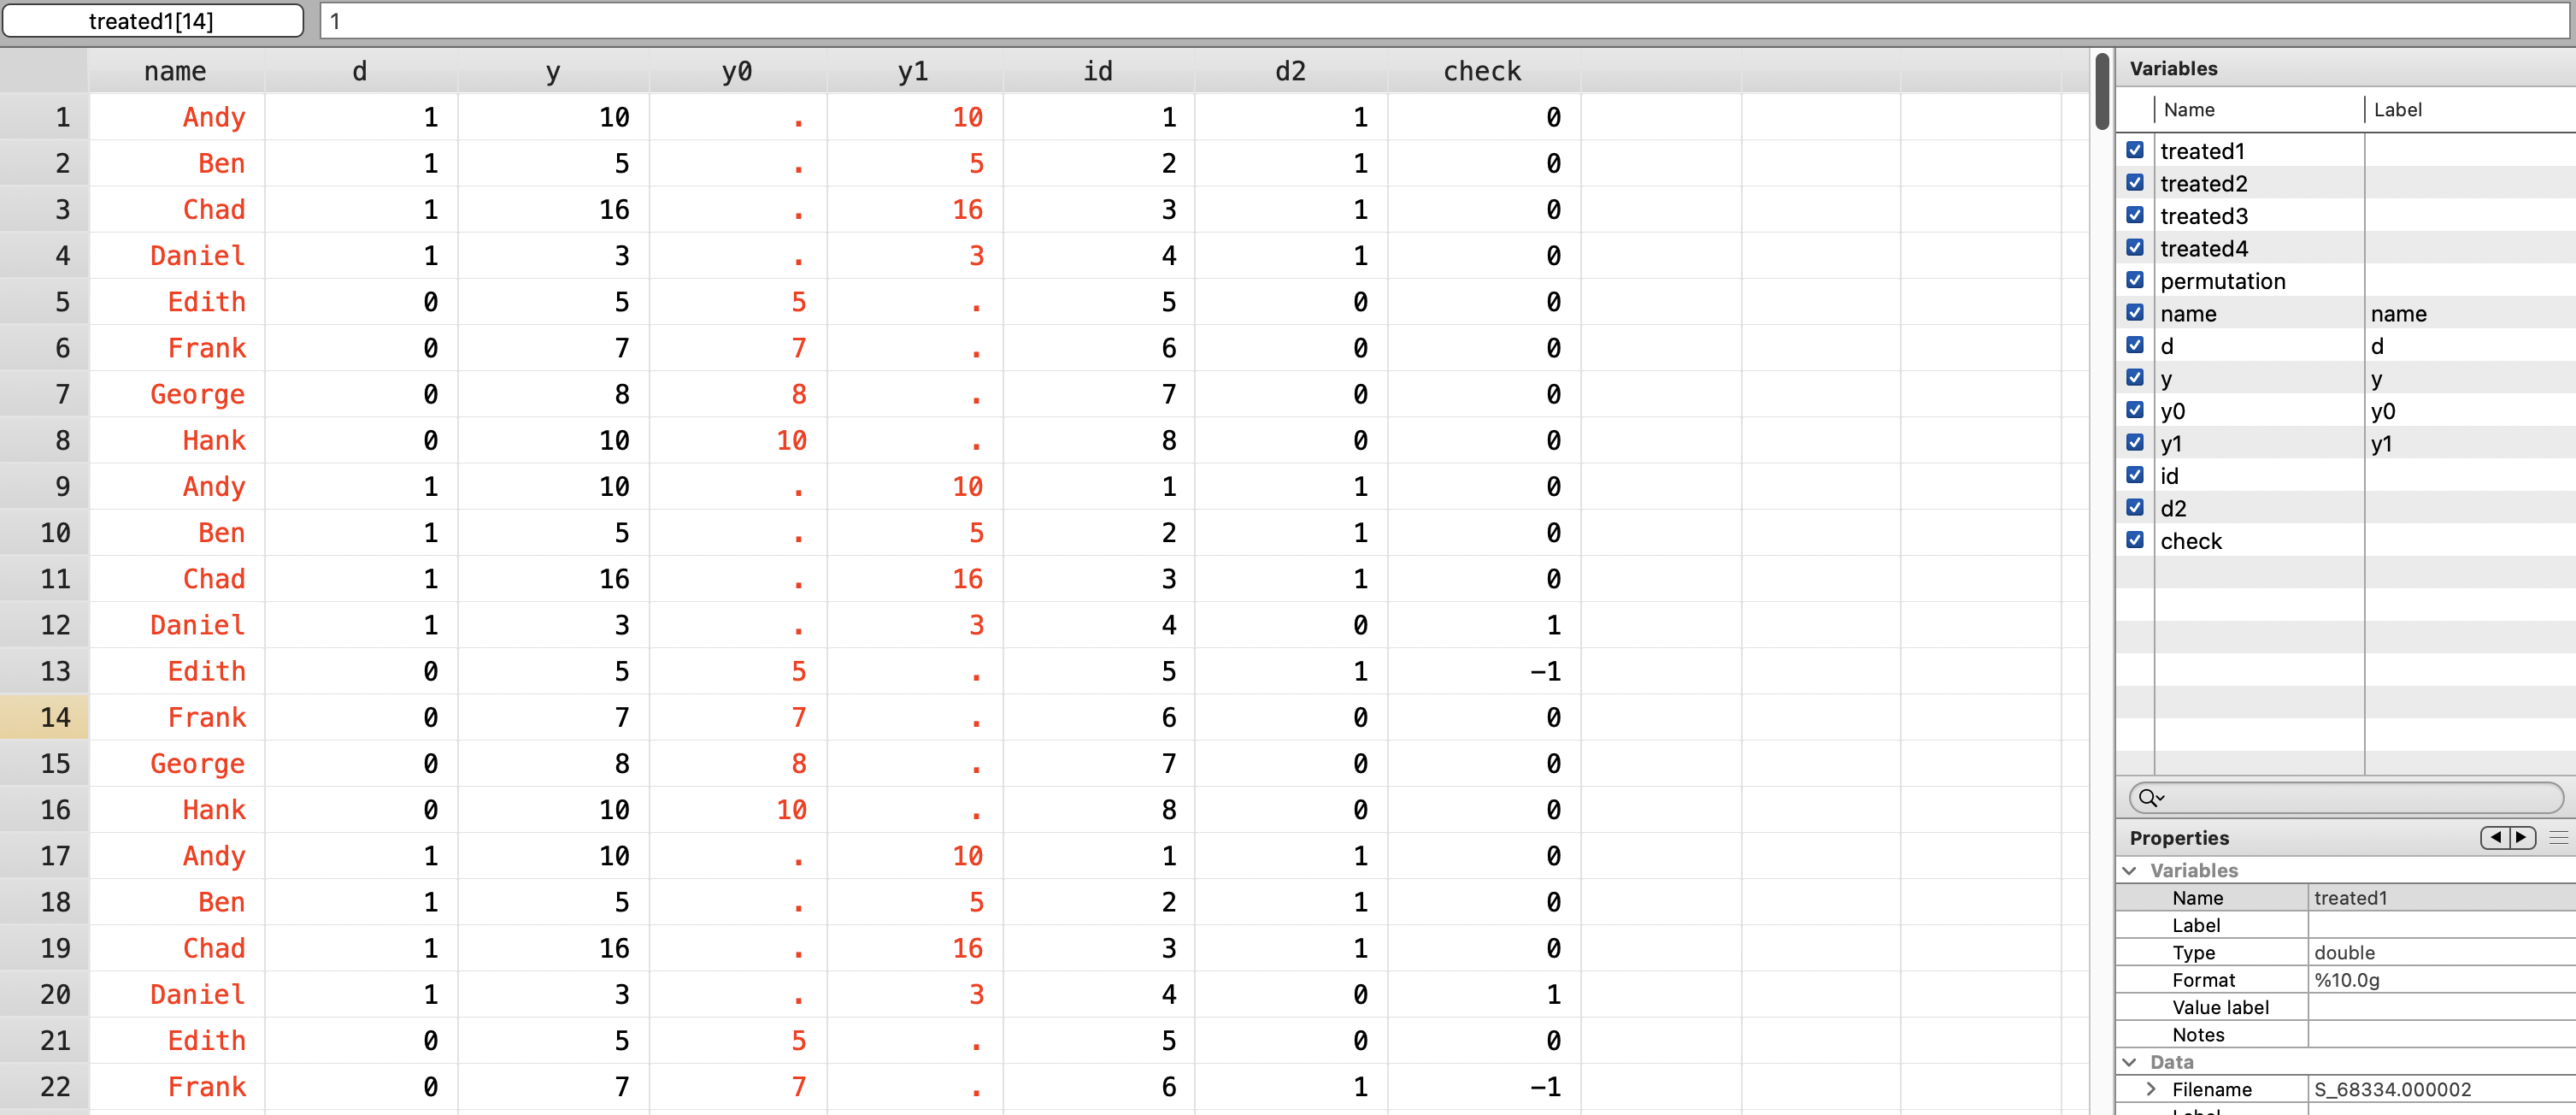
\includegraphics[keepaspectratio]{Week2_ri_example4.png}}
\caption{Set up False Treatment}
\end{figure}

Next, we will calculate true effect using absolute value of simple difference in outcomes \((SDO)\).

\begin{Shaded}
\begin{Highlighting}[]
\KeywordTok{egen}\NormalTok{ te1 = }\KeywordTok{mean}\NormalTok{(}\FunctionTok{y}\NormalTok{) }\KeywordTok{if}\NormalTok{ d2==1, }\KeywordTok{by}\NormalTok{(permutation)}
\KeywordTok{egen}\NormalTok{ te0 = }\KeywordTok{mean}\NormalTok{(}\FunctionTok{y}\NormalTok{) }\KeywordTok{if}\NormalTok{ d2==0, }\KeywordTok{by}\NormalTok{(permutation)}
\end{Highlighting}
\end{Shaded}

\begin{figure}
\centering
\pandocbounded{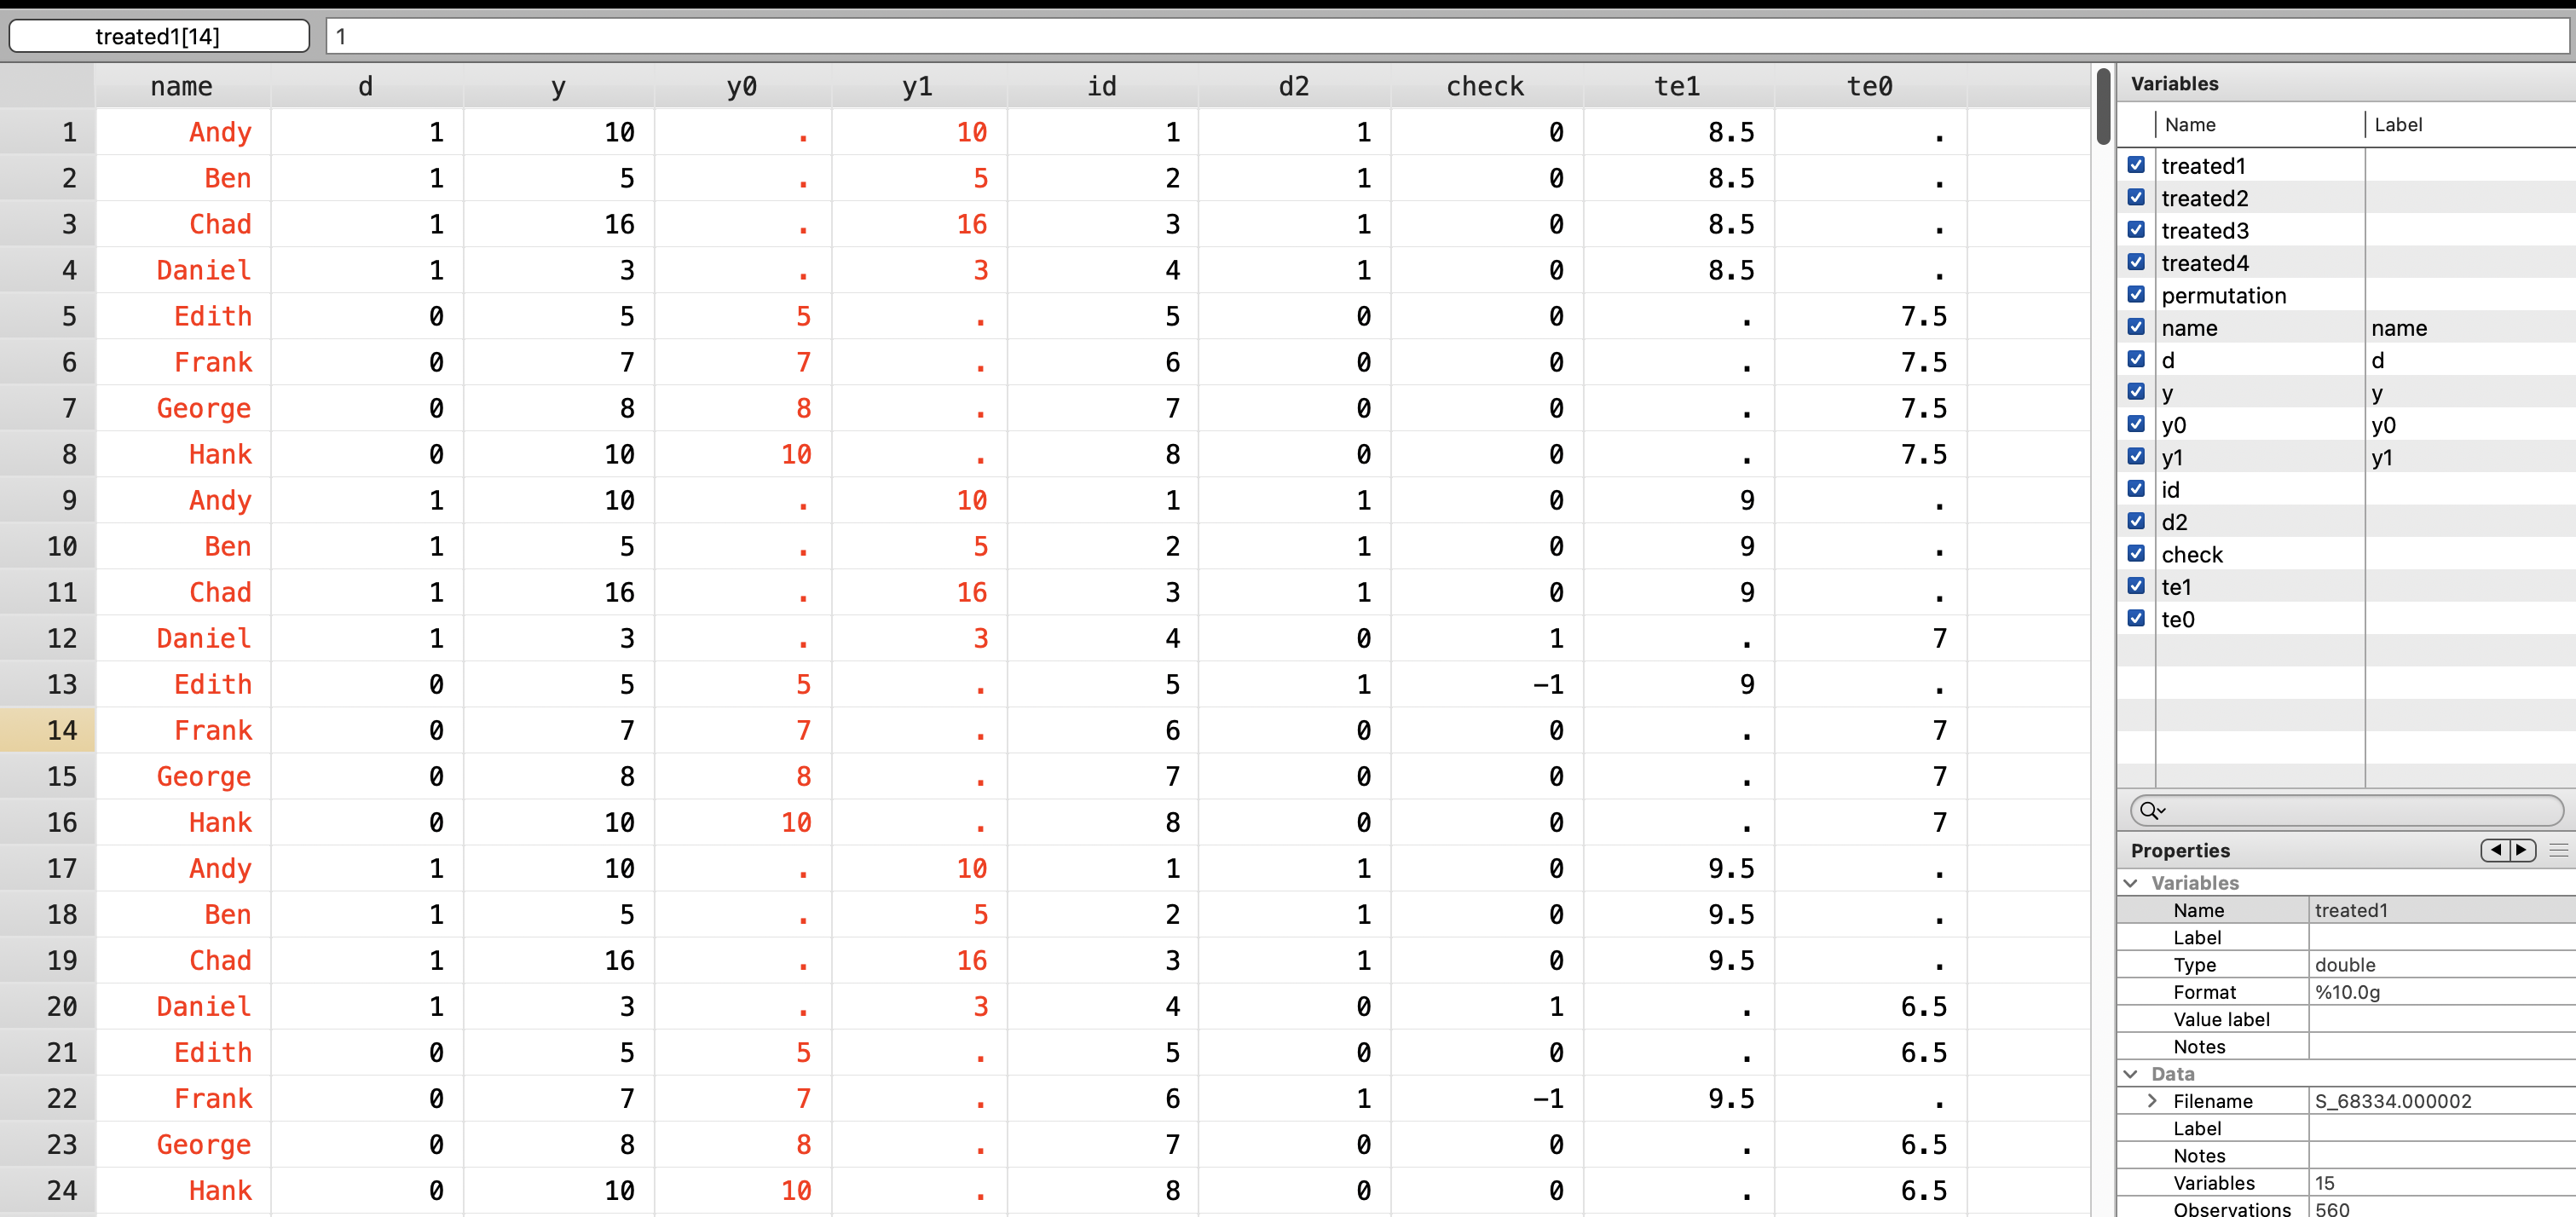
\includegraphics[keepaspectratio]{Week2_ri_example5.png}}
\caption{Get the average treatment effects by permutations}
\end{figure}

\section{Calculate the exact p-value}\label{calculate-the-exact-p-value}

Get average treatment effects \((ATE)\)

\begin{Shaded}
\begin{Highlighting}[]
\KeywordTok{collapse}\NormalTok{ (}\KeywordTok{mean}\NormalTok{) te1 te0, }\KeywordTok{by}\NormalTok{(permutation)}
\KeywordTok{gen}\NormalTok{     ate = te1 {-} te0}
\KeywordTok{keep}\NormalTok{    ate permutation}
\end{Highlighting}
\end{Shaded}

\begin{figure}
\centering
\pandocbounded{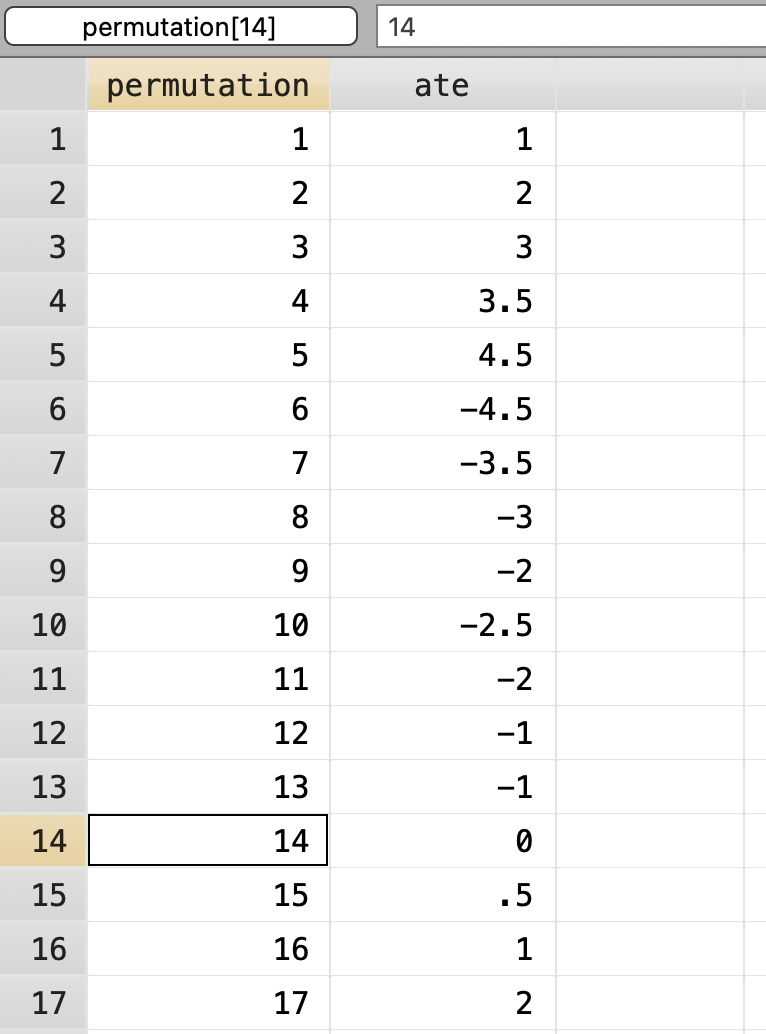
\includegraphics[keepaspectratio]{Week2_ri_example6.png}}
\caption{Collapse the treatment effects by permutation}
\end{figure}

Next, we rank the permutations

\begin{Shaded}
\begin{Highlighting}[]
\KeywordTok{gsort}\NormalTok{ {-}ate}
\KeywordTok{gen} \FunctionTok{rank}\NormalTok{ = }\DataTypeTok{\_n}
\KeywordTok{sum} \FunctionTok{rank} \KeywordTok{if}\NormalTok{ permutation==1}
\end{Highlighting}
\end{Shaded}

\begin{figure}
\centering
\pandocbounded{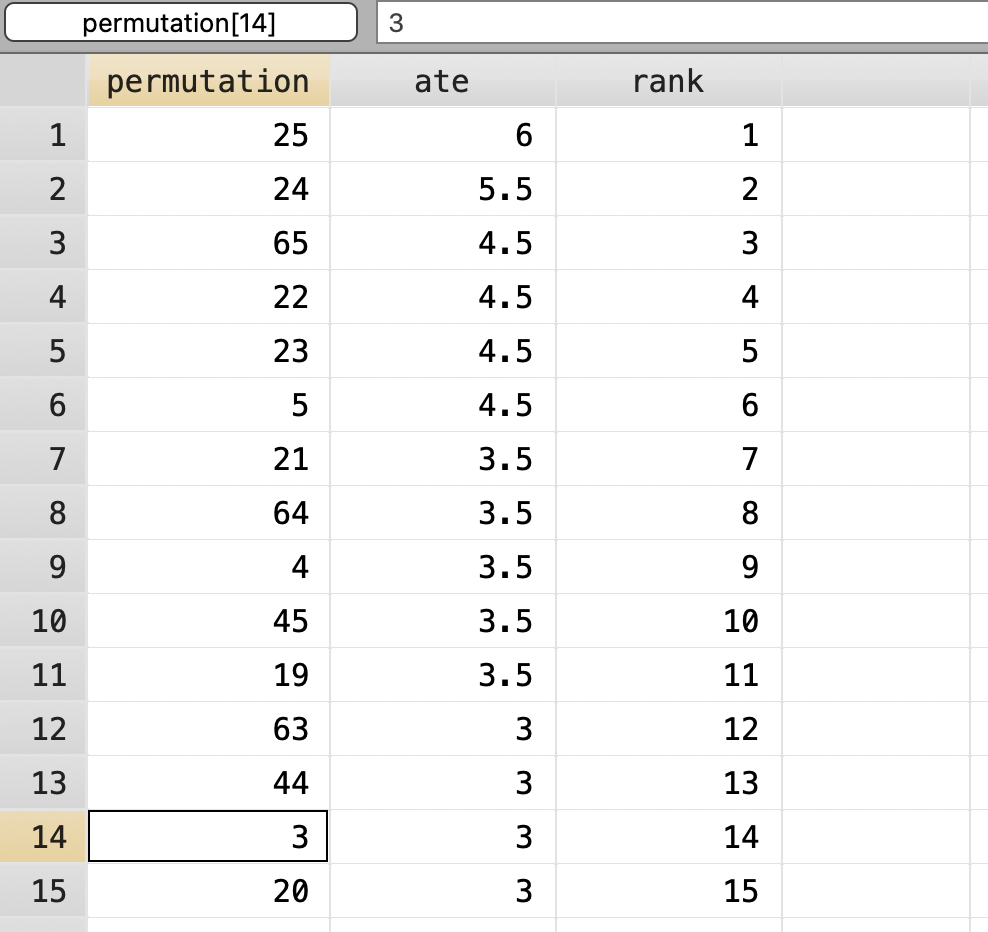
\includegraphics[keepaspectratio]{Week2_ri_example7.png}}
\caption{Sort and Rank by ATE}
\end{figure}

Finally, we calculate Exact \(p\)-value

\begin{Shaded}
\begin{Highlighting}[]
\KeywordTok{gen}\NormalTok{ pvalue = (}\OtherTok{\textasciigrave{}r(mean)\textquotesingle{}}\NormalTok{/70)}
\OtherTok{list}\NormalTok{ pvalue }\KeywordTok{if}\NormalTok{ permutation==1}
\end{Highlighting}
\end{Shaded}

\begin{verbatim}
     |    pvalue |
     |-----------|
 29. | .41428571 |
     +-----------+
\end{verbatim}

Cunningham, S. (2021). Causal Inference: The Mixtape Tape. Yale University Press

Estout. (2025). \emph{Making Regression Tables in Stata}. Retrieved from: \url{https://repec.sowi.unibe.ch/stata/estout/}

Huber, M. (2023). Causal Analysis: Impact Evaluation and Causal Machine Learning with Applications in R. The MIT Press.

Schochet, P. Z., Burghardt, J., Glazerman, S. (2001): ``National Job Corps study: The impacts of Job Corps on participants' employment and related outcomes'', Mathematica Policy Research, Washington, DC.

\bibliography{book.bib,packages.bib}

\end{document}
